\documentclass[12pt]{article}
\usepackage[T1]{fontenc}
\usepackage[utf8]{inputenc}
\usepackage[default]{sourcesanspro}
\usepackage[letterpaper,left=0.5in,right=0.5in,top=0.7in,bottom=0.7in,headheight=15pt,headsep=12pt,footskip=26pt]{geometry}
\usepackage{fancyhdr}
\usepackage{tikz}
\pagestyle{fancy}
\fancyhf{}
\fancyhead[L]{Week 10 / Bridges / K--1}
\fancyfoot[L]{Bellingham Math Circle / Week 10 / F10-K-v4}
\fancyfoot[R]{\thepage}
\renewcommand{\headrulewidth}{0.4pt}
\renewcommand{\footrulewidth}{0pt}
\setlength{\parindent}{0pt}
\setlength{\parskip}{0pt}
\raggedright
\raggedbottom
\hyphenpenalty=10000
\exhyphenpenalty=10000
\frenchspacing
\newcommand{\prob}[1]{\textbf{Problem #1:}\ }
\tikzset{
  bandout/.style={line width=1.6cm, draw=black!75, line cap=butt},
  bandfill/.style={line width=1.480cm, draw=black!9, line cap=butt},
  island/.style={fill=white, draw=black, line width=1.3pt},
  islandlabel/.style={font=\sffamily\Large},
  stroke/.style={line width=1.4pt, draw=black!50, line cap=round, line join=round},
}

\begin{document}
\large

Put a counter on every bridge, and put your token on an island. The token moves by crossing bridges. Each time it crosses a bridge, pick up that bridge's counter. A bridge with no counter cannot be crossed.

\vspace{6mm}

\begin{minipage}{\linewidth}\raggedright
\prob{1}Pick up every counter in each town. Color the island where you started.

\vspace{5mm}\noindent 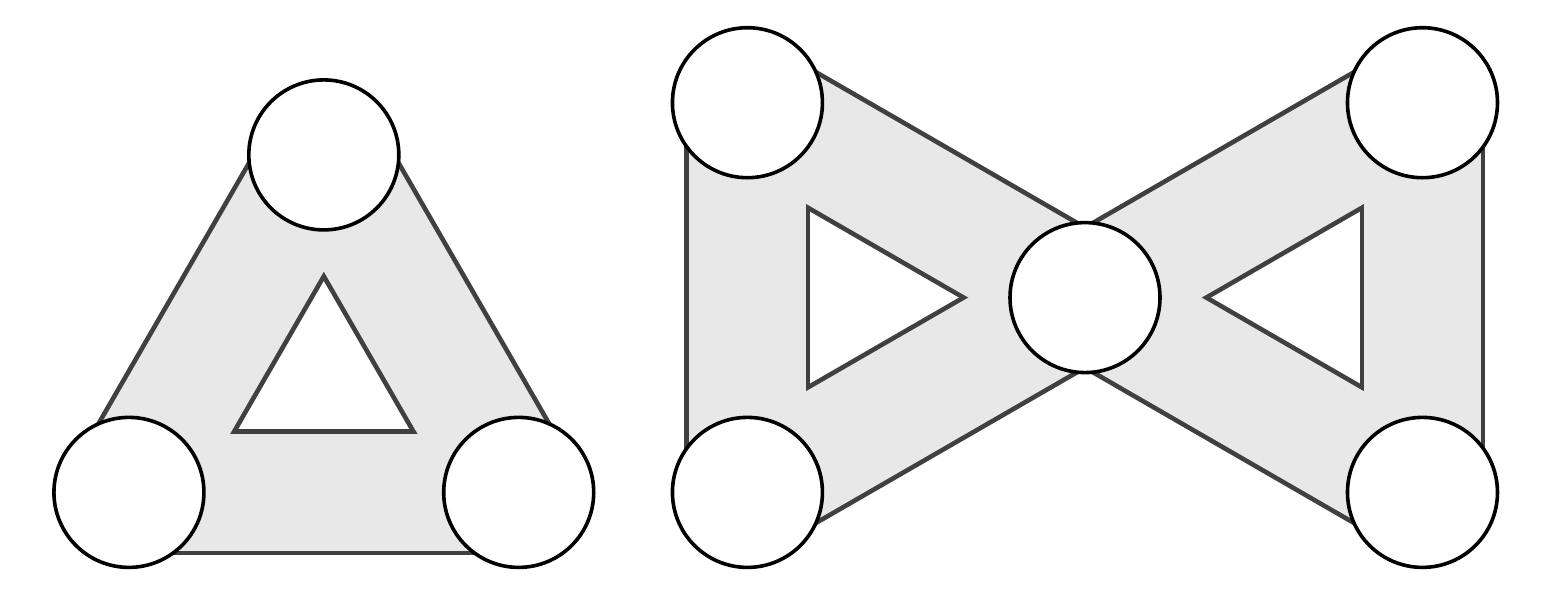
\begin{tikzpicture}
\useasboundingbox (0,0) rectangle (19.0,6.855);
\draw[bandout] (1.286,0.953) -- (6.236,0.953);
\draw[bandout] (6.236,0.953) -- (3.761,5.239);
\draw[bandout] (3.761,5.239) -- (1.286,0.953);
\draw[bandfill] (1.286,0.953) -- (6.236,0.953);
\draw[bandfill] (6.236,0.953) -- (3.761,5.239);
\draw[bandfill] (3.761,5.239) -- (1.286,0.953);
\draw[island] (1.286,0.953) circle (0.9525);
\draw[island] (6.236,0.953) circle (0.9525);
\draw[island] (3.761,5.239) circle (0.9525);
\draw[bandout] (13.428,3.427) -- (9.141,5.902);
\draw[bandout] (9.141,5.902) -- (9.141,0.953);
\draw[bandout] (9.141,0.953) -- (13.428,3.427);
\draw[bandout] (13.428,3.427) -- (17.714,5.902);
\draw[bandout] (17.714,5.902) -- (17.714,0.953);
\draw[bandout] (17.714,0.953) -- (13.428,3.427);
\draw[bandfill] (13.428,3.427) -- (9.141,5.902);
\draw[bandfill] (9.141,5.902) -- (9.141,0.953);
\draw[bandfill] (9.141,0.953) -- (13.428,3.427);
\draw[bandfill] (13.428,3.427) -- (17.714,5.902);
\draw[bandfill] (17.714,5.902) -- (17.714,0.953);
\draw[bandfill] (17.714,0.953) -- (13.428,3.427);
\draw[island] (9.141,5.902) circle (0.9525);
\draw[island] (9.141,0.953) circle (0.9525);
\draw[island] (13.428,3.427) circle (0.9525);
\draw[island] (17.714,5.902) circle (0.9525);
\draw[island] (17.714,0.953) circle (0.9525);
\end{tikzpicture}
\end{minipage}


\par\vspace{7mm}\noindent 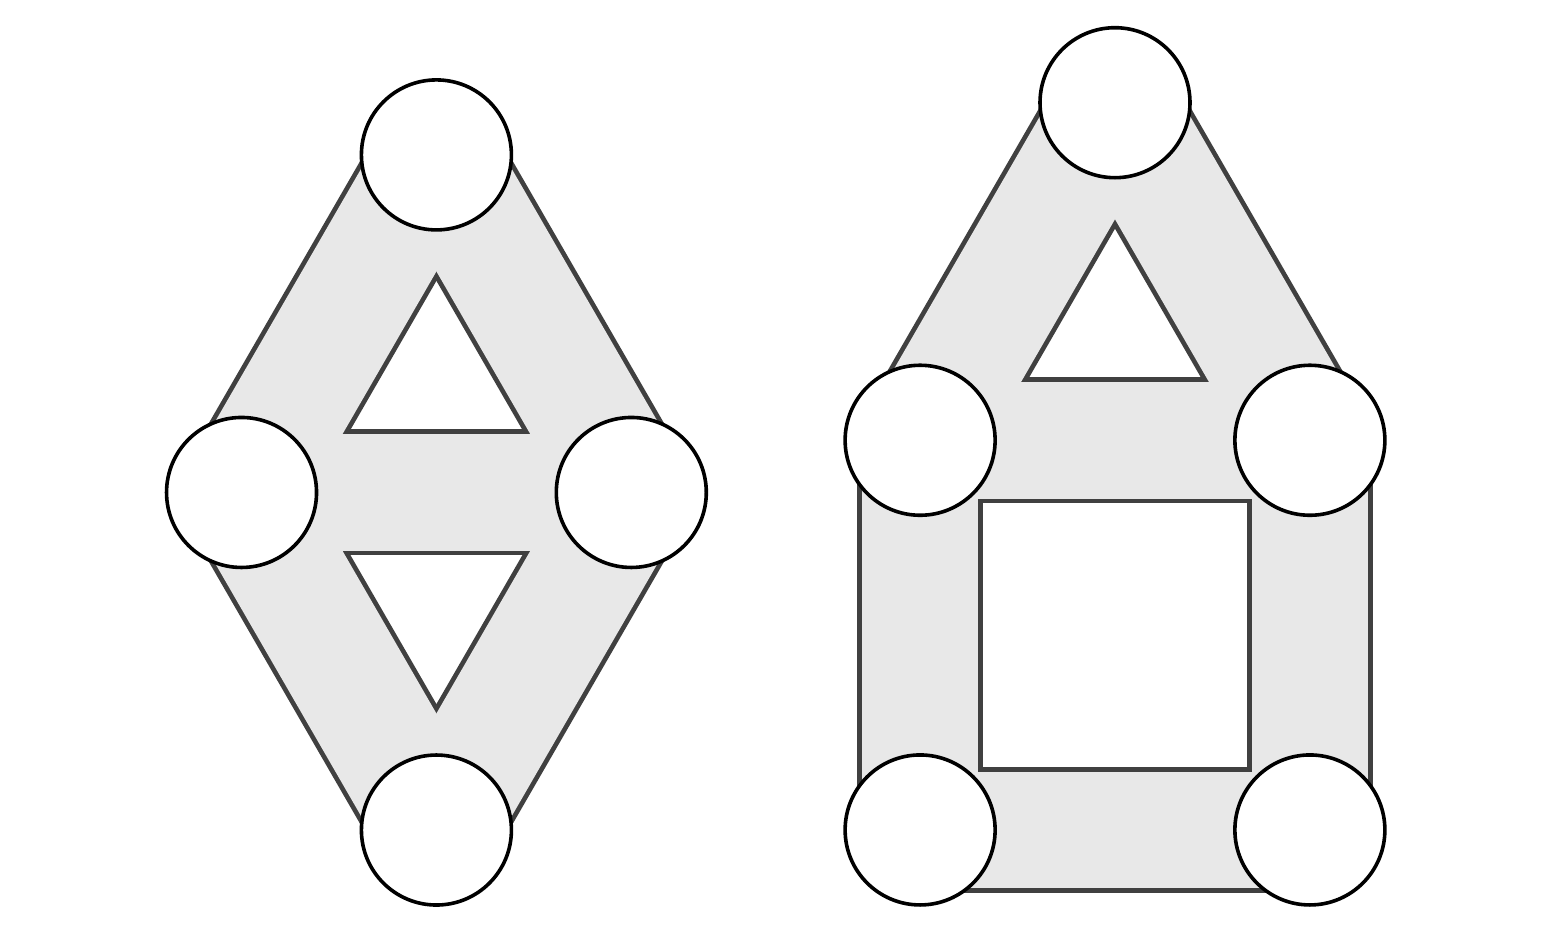
\begin{tikzpicture}
\useasboundingbox (0,0) rectangle (19.0,11.142);
\draw[bandout] (2.716,5.239) -- (7.666,5.239);
\draw[bandout] (2.716,5.239) -- (5.191,9.526);
\draw[bandout] (7.666,5.239) -- (5.191,9.526);
\draw[bandout] (2.716,5.239) -- (5.191,0.952);
\draw[bandout] (7.666,5.239) -- (5.191,0.952);
\draw[bandfill] (2.716,5.239) -- (7.666,5.239);
\draw[bandfill] (2.716,5.239) -- (5.191,9.526);
\draw[bandfill] (7.666,5.239) -- (5.191,9.526);
\draw[bandfill] (2.716,5.239) -- (5.191,0.952);
\draw[bandfill] (7.666,5.239) -- (5.191,0.952);
\draw[island] (5.191,9.526) circle (0.9525);
\draw[island] (2.716,5.239) circle (0.9525);
\draw[island] (7.666,5.239) circle (0.9525);
\draw[island] (5.191,0.952) circle (0.9525);
\draw[bandout] (11.334,0.953) -- (16.284,0.953);
\draw[bandout] (16.284,0.953) -- (16.284,5.902);
\draw[bandout] (16.284,5.902) -- (11.334,5.902);
\draw[bandout] (11.334,5.902) -- (11.334,0.953);
\draw[bandout] (11.334,5.902) -- (13.809,10.189);
\draw[bandout] (13.809,10.189) -- (16.284,5.902);
\draw[bandfill] (11.334,0.953) -- (16.284,0.953);
\draw[bandfill] (16.284,0.953) -- (16.284,5.902);
\draw[bandfill] (16.284,5.902) -- (11.334,5.902);
\draw[bandfill] (11.334,5.902) -- (11.334,0.953);
\draw[bandfill] (11.334,5.902) -- (13.809,10.189);
\draw[bandfill] (13.809,10.189) -- (16.284,5.902);
\draw[island] (11.334,0.953) circle (0.9525);
\draw[island] (16.284,0.953) circle (0.9525);
\draw[island] (16.284,5.902) circle (0.9525);
\draw[island] (11.334,5.902) circle (0.9525);
\draw[island] (13.809,10.189) circle (0.9525);
\end{tikzpicture}


\par\vspace{9mm}

\newpage

\begin{minipage}{\linewidth}\raggedright
\prob{2}Color every island where your token can start and still pick up every counter.

\vspace{5mm}\noindent 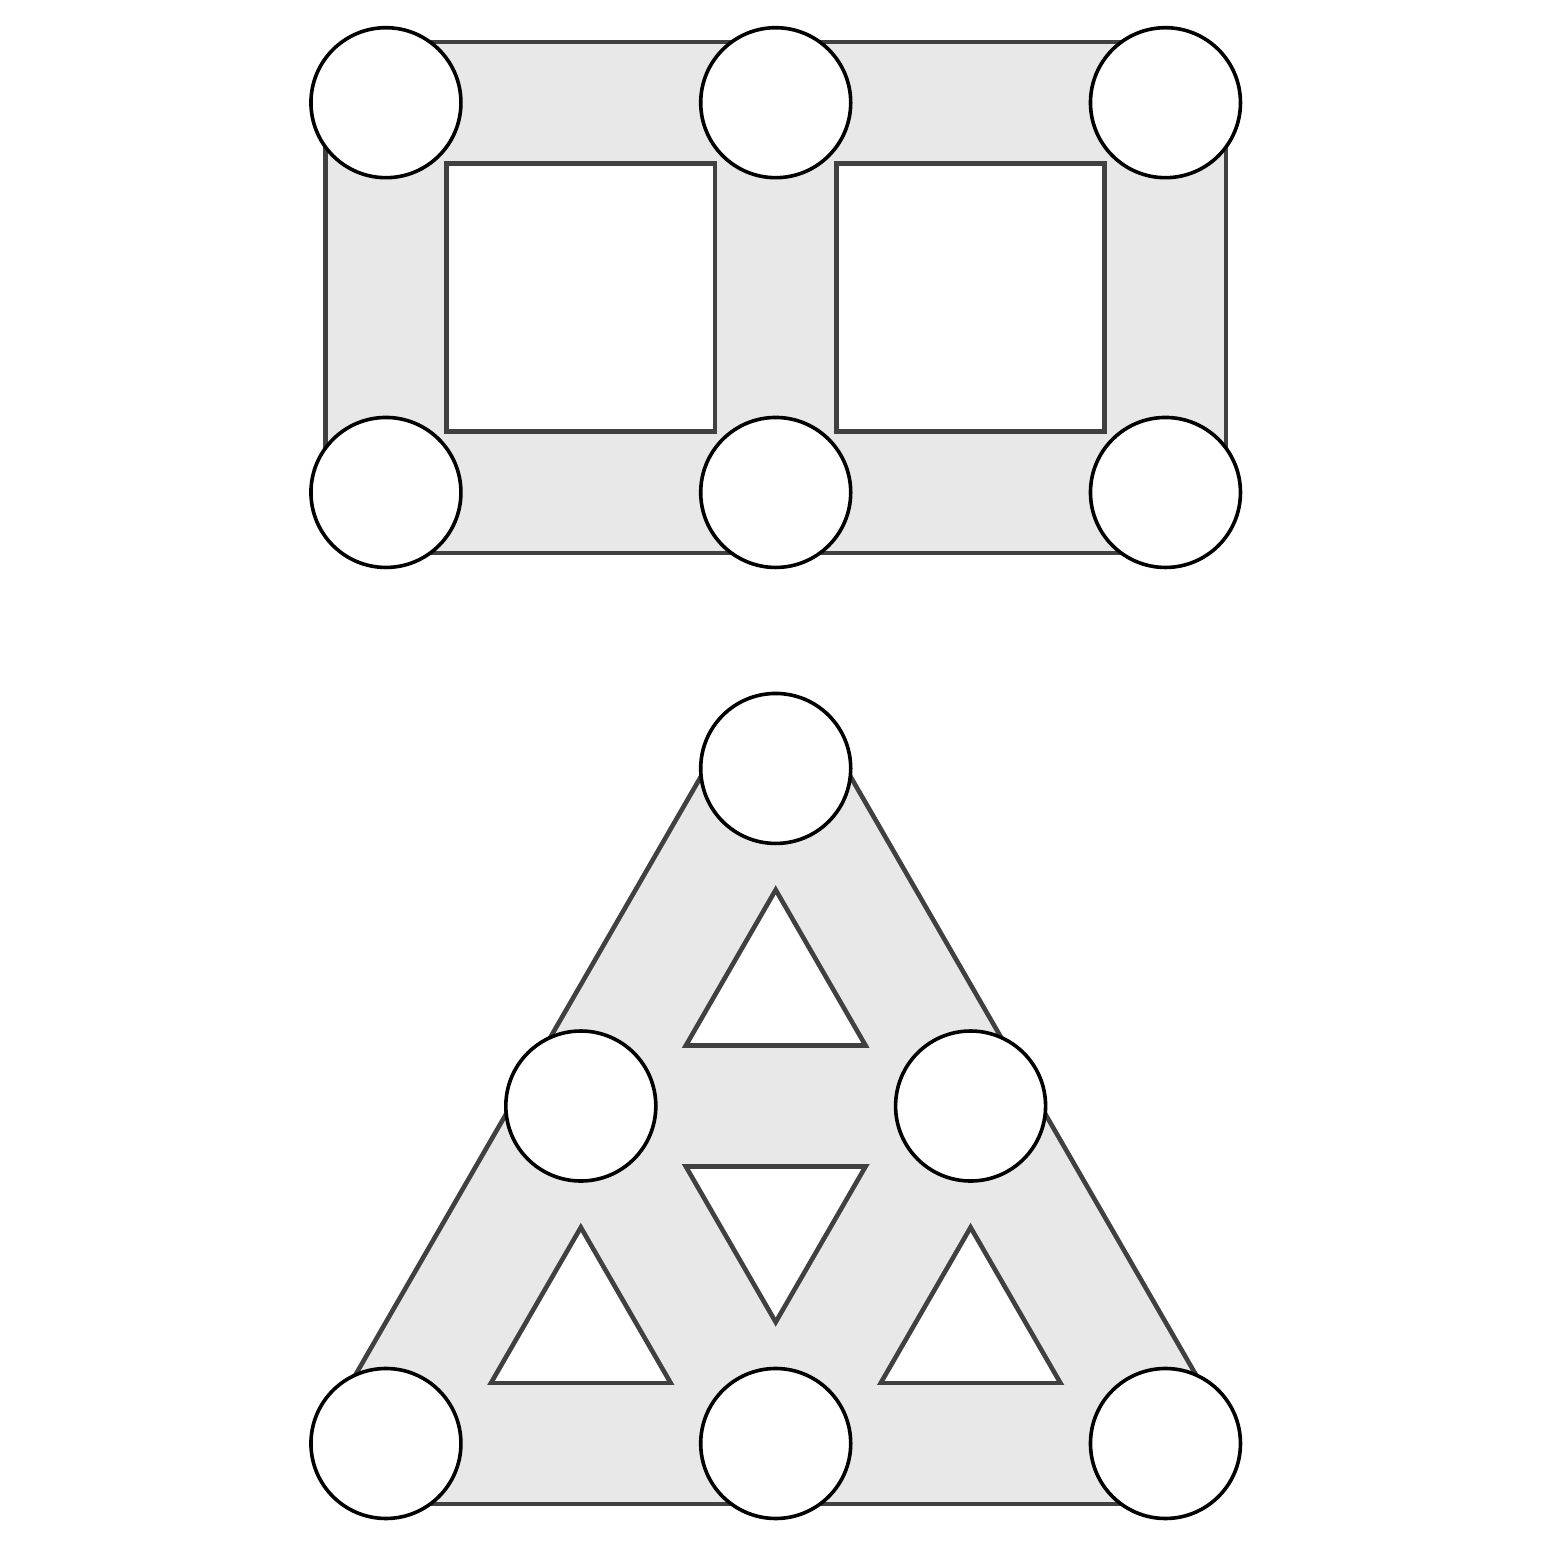
\begin{tikzpicture}
\useasboundingbox (0,0) rectangle (19.0,18.934);
\draw[bandout] (4.550,13.031) -- (9.500,13.031);
\draw[bandout] (4.550,17.981) -- (9.500,17.981);
\draw[bandout] (9.500,13.031) -- (14.450,13.031);
\draw[bandout] (9.500,17.981) -- (14.450,17.981);
\draw[bandout] (4.550,13.031) -- (4.550,17.981);
\draw[bandout] (9.500,13.031) -- (9.500,17.981);
\draw[bandout] (14.450,13.031) -- (14.450,17.981);
\draw[bandfill] (4.550,13.031) -- (9.500,13.031);
\draw[bandfill] (4.550,17.981) -- (9.500,17.981);
\draw[bandfill] (9.500,13.031) -- (14.450,13.031);
\draw[bandfill] (9.500,17.981) -- (14.450,17.981);
\draw[bandfill] (4.550,13.031) -- (4.550,17.981);
\draw[bandfill] (9.500,13.031) -- (9.500,17.981);
\draw[bandfill] (14.450,13.031) -- (14.450,17.981);
\draw[island] (4.550,13.031) circle (0.9525);
\draw[island] (9.500,13.031) circle (0.9525);
\draw[island] (14.450,13.031) circle (0.9525);
\draw[island] (4.550,17.981) circle (0.9525);
\draw[island] (9.500,17.981) circle (0.9525);
\draw[island] (14.450,17.981) circle (0.9525);
\draw[bandout] (4.550,0.953) -- (9.500,0.953);
\draw[bandout] (9.500,0.953) -- (14.450,0.953);
\draw[bandout] (14.450,0.953) -- (11.975,5.239);
\draw[bandout] (11.975,5.239) -- (9.500,9.526);
\draw[bandout] (9.500,9.526) -- (7.025,5.239);
\draw[bandout] (7.025,5.239) -- (4.550,0.953);
\draw[bandout] (9.500,0.953) -- (11.975,5.239);
\draw[bandout] (11.975,5.239) -- (7.025,5.239);
\draw[bandout] (7.025,5.239) -- (9.500,0.953);
\draw[bandfill] (4.550,0.953) -- (9.500,0.953);
\draw[bandfill] (9.500,0.953) -- (14.450,0.953);
\draw[bandfill] (14.450,0.953) -- (11.975,5.239);
\draw[bandfill] (11.975,5.239) -- (9.500,9.526);
\draw[bandfill] (9.500,9.526) -- (7.025,5.239);
\draw[bandfill] (7.025,5.239) -- (4.550,0.953);
\draw[bandfill] (9.500,0.953) -- (11.975,5.239);
\draw[bandfill] (11.975,5.239) -- (7.025,5.239);
\draw[bandfill] (7.025,5.239) -- (9.500,0.953);
\draw[island] (4.550,0.953) circle (0.9525);
\draw[island] (9.500,0.953) circle (0.9525);
\draw[island] (14.450,0.953) circle (0.9525);
\draw[island] (7.025,5.239) circle (0.9525);
\draw[island] (11.975,5.239) circle (0.9525);
\draw[island] (9.500,9.526) circle (0.9525);
\end{tikzpicture}
\end{minipage}


\par\vspace{9mm}

\newpage

\begin{minipage}{\linewidth}\raggedright
\prob{3}Can you pick up every counter? Put a check in the box if you can and an X if you cannot.

\vspace{5mm}\noindent 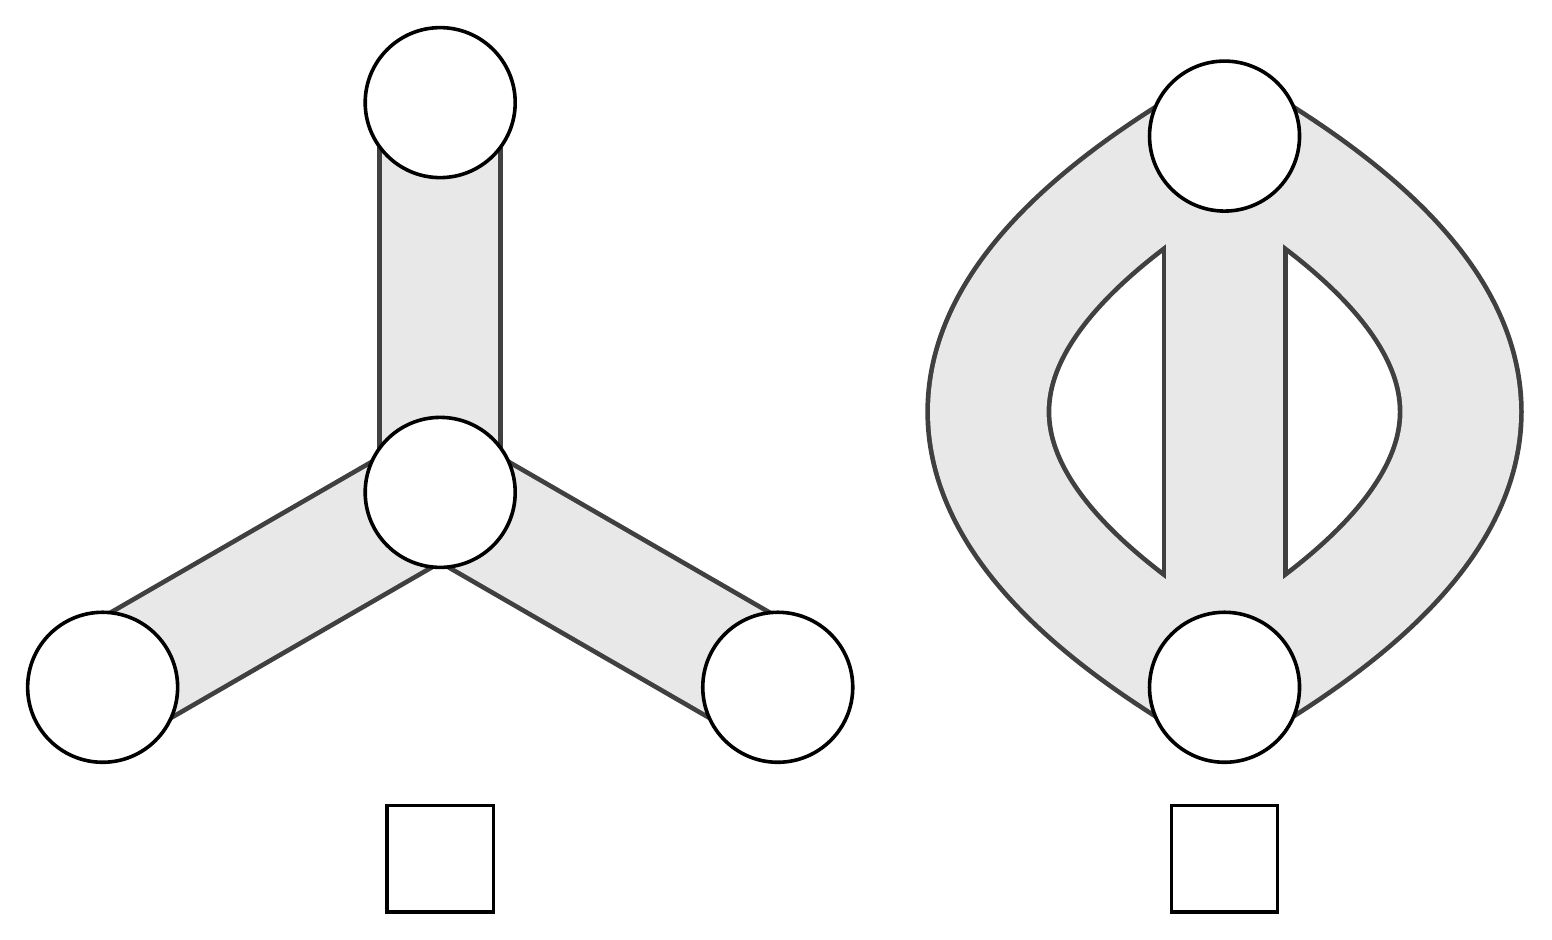
\begin{tikzpicture}
\useasboundingbox (0,0) rectangle (19.0,11.230);
\draw[bandout] (5.239,5.328) -- (5.239,10.278);
\draw[bandout] (5.239,5.328) -- (0.952,2.853);
\draw[bandout] (5.239,5.328) -- (9.526,2.853);
\draw[bandfill] (5.239,5.328) -- (5.239,10.278);
\draw[bandfill] (5.239,5.328) -- (0.952,2.853);
\draw[bandfill] (5.239,5.328) -- (9.526,2.853);
\draw[island] (5.239,5.328) circle (0.9525);
\draw[island] (5.239,10.278) circle (0.9525);
\draw[island] (0.952,2.853) circle (0.9525);
\draw[island] (9.526,2.853) circle (0.9525);
\draw[line width=1.2pt] (4.564,0.000) rectangle ++(1.35,1.35);
\draw[bandout] (15.200,2.853) -- (15.200,9.853);
\draw[bandout] (15.200,2.853) .. controls (11.200,5.186) and (11.200,7.519) .. (15.200,9.853);
\draw[bandout] (15.200,2.853) .. controls (19.200,5.186) and (19.200,7.519) .. (15.200,9.853);
\draw[bandfill] (15.200,2.853) -- (15.200,9.853);
\draw[bandfill] (15.200,2.853) .. controls (11.200,5.186) and (11.200,7.519) .. (15.200,9.853);
\draw[bandfill] (15.200,2.853) .. controls (19.200,5.186) and (19.200,7.519) .. (15.200,9.853);
\draw[island] (15.200,2.853) circle (0.9525);
\draw[island] (15.200,9.853) circle (0.9525);
\draw[line width=1.2pt] (14.525,0.000) rectangle ++(1.35,1.35);
\end{tikzpicture}
\end{minipage}


\par\vspace{7mm}\noindent 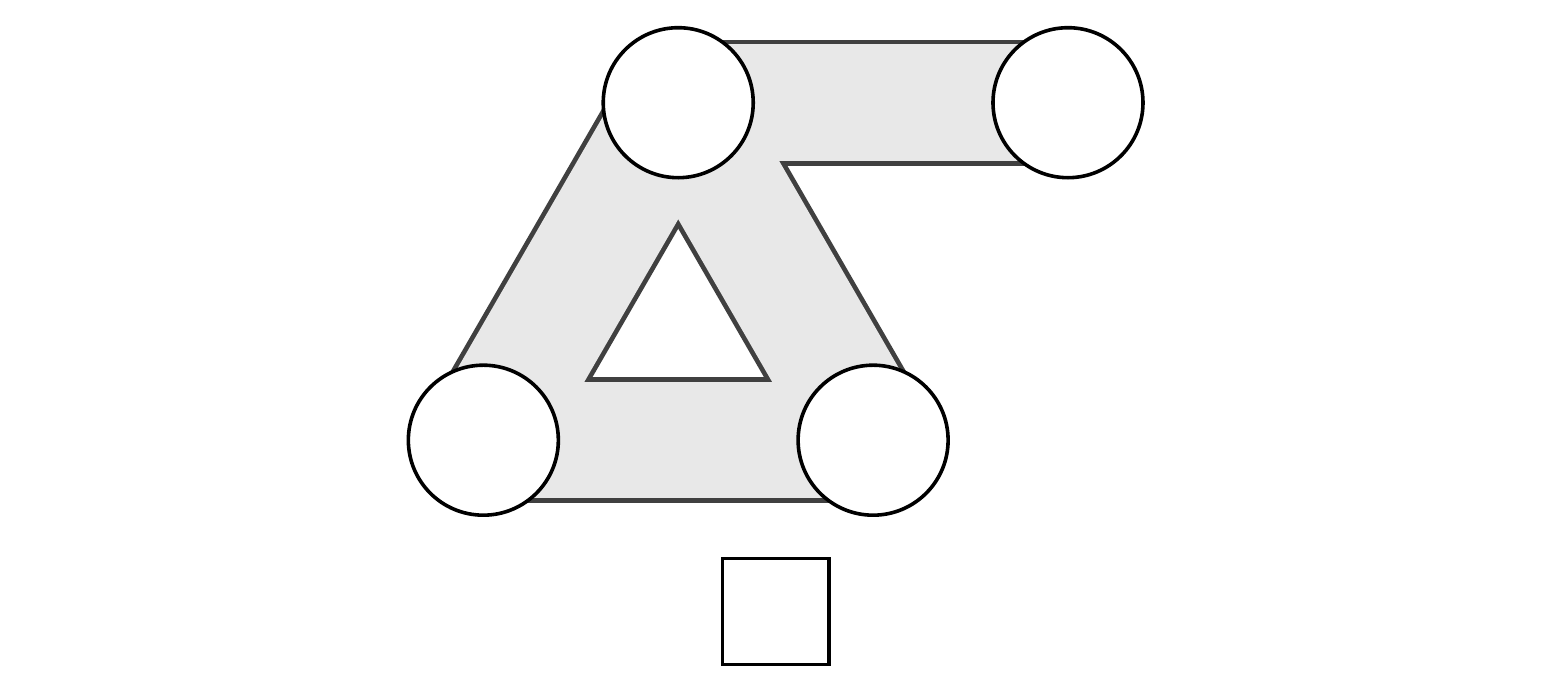
\begin{tikzpicture}
\useasboundingbox (0,0) rectangle (19.0,8.092);
\draw[bandout] (5.787,2.853) -- (10.737,2.853);
\draw[bandout] (10.737,2.853) -- (8.262,7.139);
\draw[bandout] (8.262,7.139) -- (5.787,2.853);
\draw[bandout] (8.262,7.139) -- (13.212,7.139);
\draw[bandfill] (5.787,2.853) -- (10.737,2.853);
\draw[bandfill] (10.737,2.853) -- (8.262,7.139);
\draw[bandfill] (8.262,7.139) -- (5.787,2.853);
\draw[bandfill] (8.262,7.139) -- (13.212,7.139);
\draw[island] (5.787,2.853) circle (0.9525);
\draw[island] (10.737,2.853) circle (0.9525);
\draw[island] (8.262,7.139) circle (0.9525);
\draw[island] (13.212,7.139) circle (0.9525);
\draw[line width=1.2pt] (8.825,0.000) rectangle ++(1.35,1.35);
\end{tikzpicture}


\par\vspace{7mm}\noindent 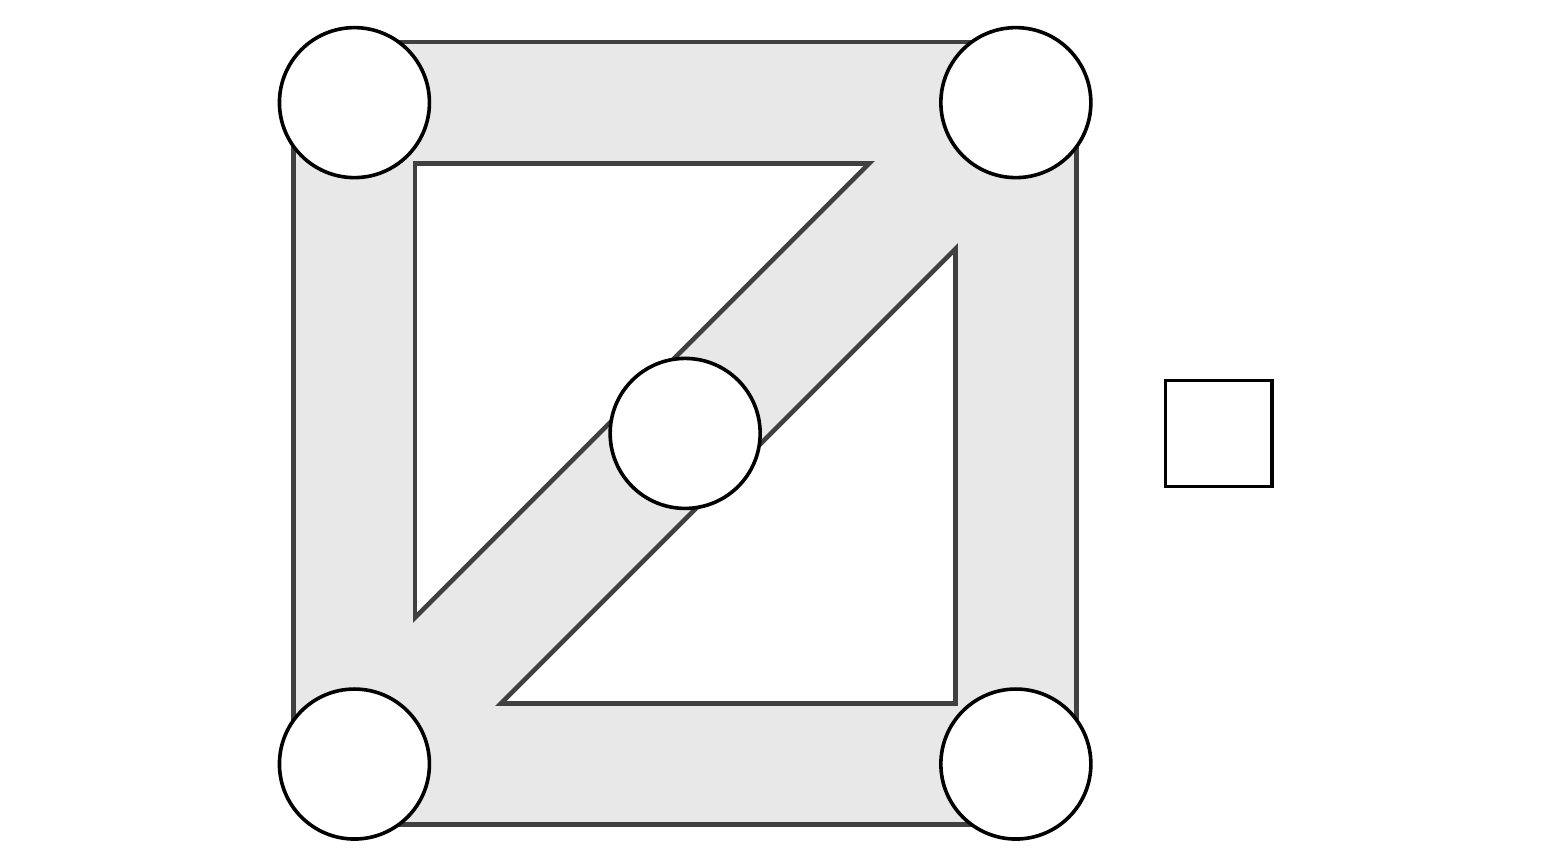
\begin{tikzpicture}
\useasboundingbox (0,0) rectangle (19.0,10.305);
\draw[bandout] (4.150,0.953) -- (12.550,0.953);
\draw[bandout] (12.550,0.953) -- (12.550,9.353);
\draw[bandout] (12.550,9.353) -- (4.150,9.353);
\draw[bandout] (4.150,9.353) -- (4.150,0.953);
\draw[bandout] (8.350,5.152) -- (4.150,0.953);
\draw[bandout] (8.350,5.152) -- (12.550,9.353);
\draw[bandfill] (4.150,0.953) -- (12.550,0.953);
\draw[bandfill] (12.550,0.953) -- (12.550,9.353);
\draw[bandfill] (12.550,9.353) -- (4.150,9.353);
\draw[bandfill] (4.150,9.353) -- (4.150,0.953);
\draw[bandfill] (8.350,5.152) -- (4.150,0.953);
\draw[bandfill] (8.350,5.152) -- (12.550,9.353);
\draw[island] (4.150,0.953) circle (0.9525);
\draw[island] (12.550,0.953) circle (0.9525);
\draw[island] (12.550,9.353) circle (0.9525);
\draw[island] (4.150,9.353) circle (0.9525);
\draw[island] (8.350,5.152) circle (0.9525);
\draw[line width=1.2pt] (14.453,4.478) rectangle ++(1.35,1.35);
\end{tikzpicture}


\par\vspace{7mm}\noindent 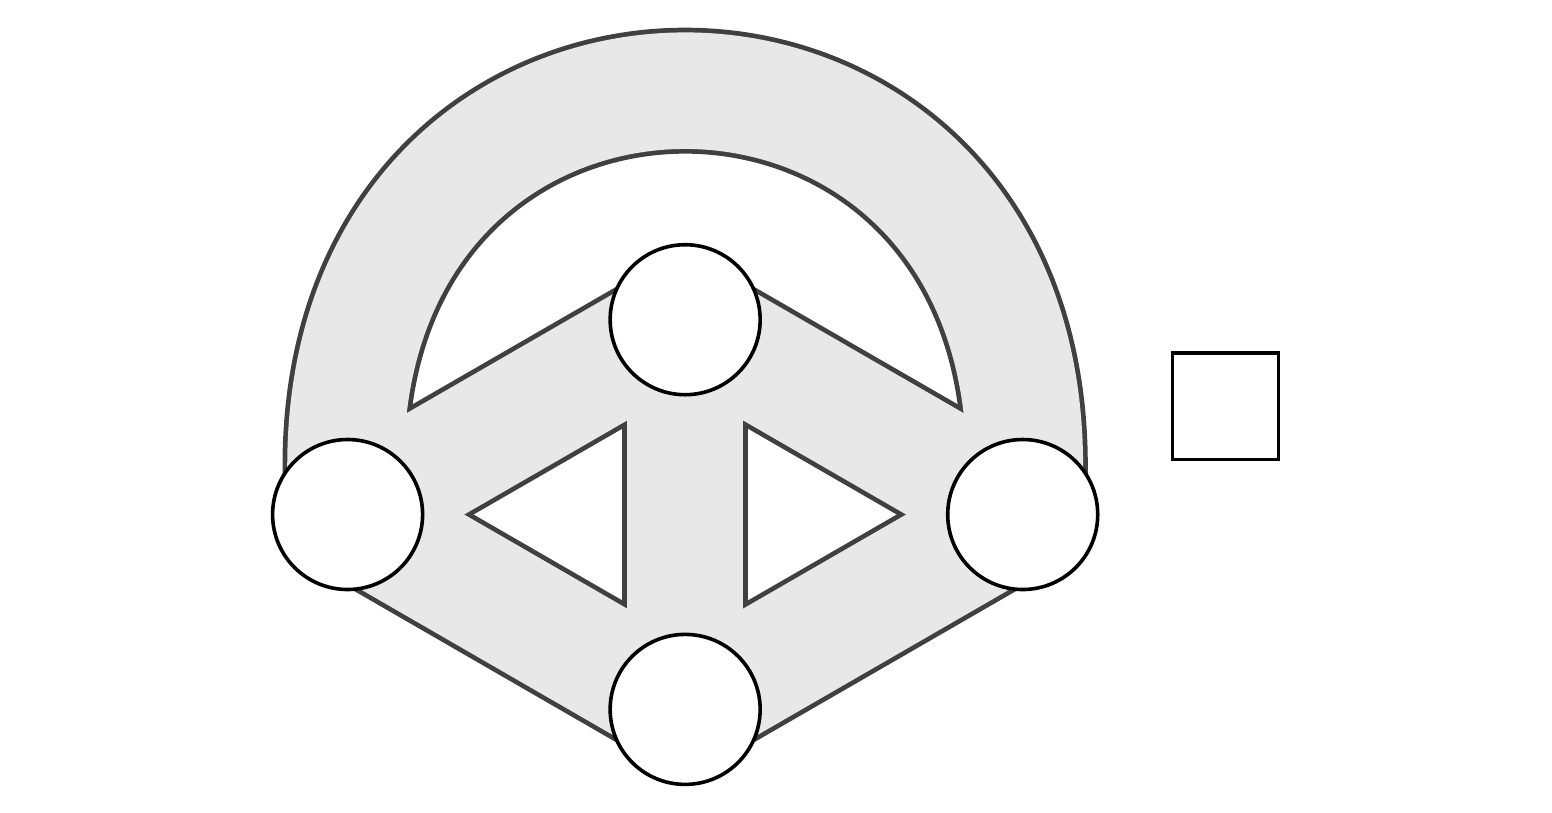
\begin{tikzpicture}
\useasboundingbox (0,0) rectangle (19.0,9.611);
\draw[bandout] (8.350,5.902) -- (8.350,0.953);
\draw[bandout] (8.350,5.902) -- (4.063,3.428);
\draw[bandout] (8.350,5.902) -- (12.637,3.428);
\draw[bandout] (8.350,0.953) -- (4.063,3.428);
\draw[bandout] (8.350,0.953) -- (12.637,3.428);
\draw[bandout] (4.063,3.428) .. controls (3.463,10.605) and (13.237,10.605) .. (12.637,3.428);
\draw[bandfill] (8.350,5.902) -- (8.350,0.953);
\draw[bandfill] (8.350,5.902) -- (4.063,3.428);
\draw[bandfill] (8.350,5.902) -- (12.637,3.428);
\draw[bandfill] (8.350,0.953) -- (4.063,3.428);
\draw[bandfill] (8.350,0.953) -- (12.637,3.428);
\draw[bandfill] (4.063,3.428) .. controls (3.463,10.605) and (13.237,10.605) .. (12.637,3.428);
\draw[island] (8.350,5.902) circle (0.9525);
\draw[island] (8.350,0.953) circle (0.9525);
\draw[island] (4.063,3.428) circle (0.9525);
\draw[island] (12.637,3.428) circle (0.9525);
\draw[line width=1.2pt] (14.539,4.130) rectangle ++(1.35,1.35);
\end{tikzpicture}


\par\vspace{9mm}

\newpage

\begin{minipage}{\linewidth}\raggedright
\prob{4}Pick up every counter and end on the island where you started. Put a check in the box if you can and an X if you cannot.

\vspace{5mm}\noindent 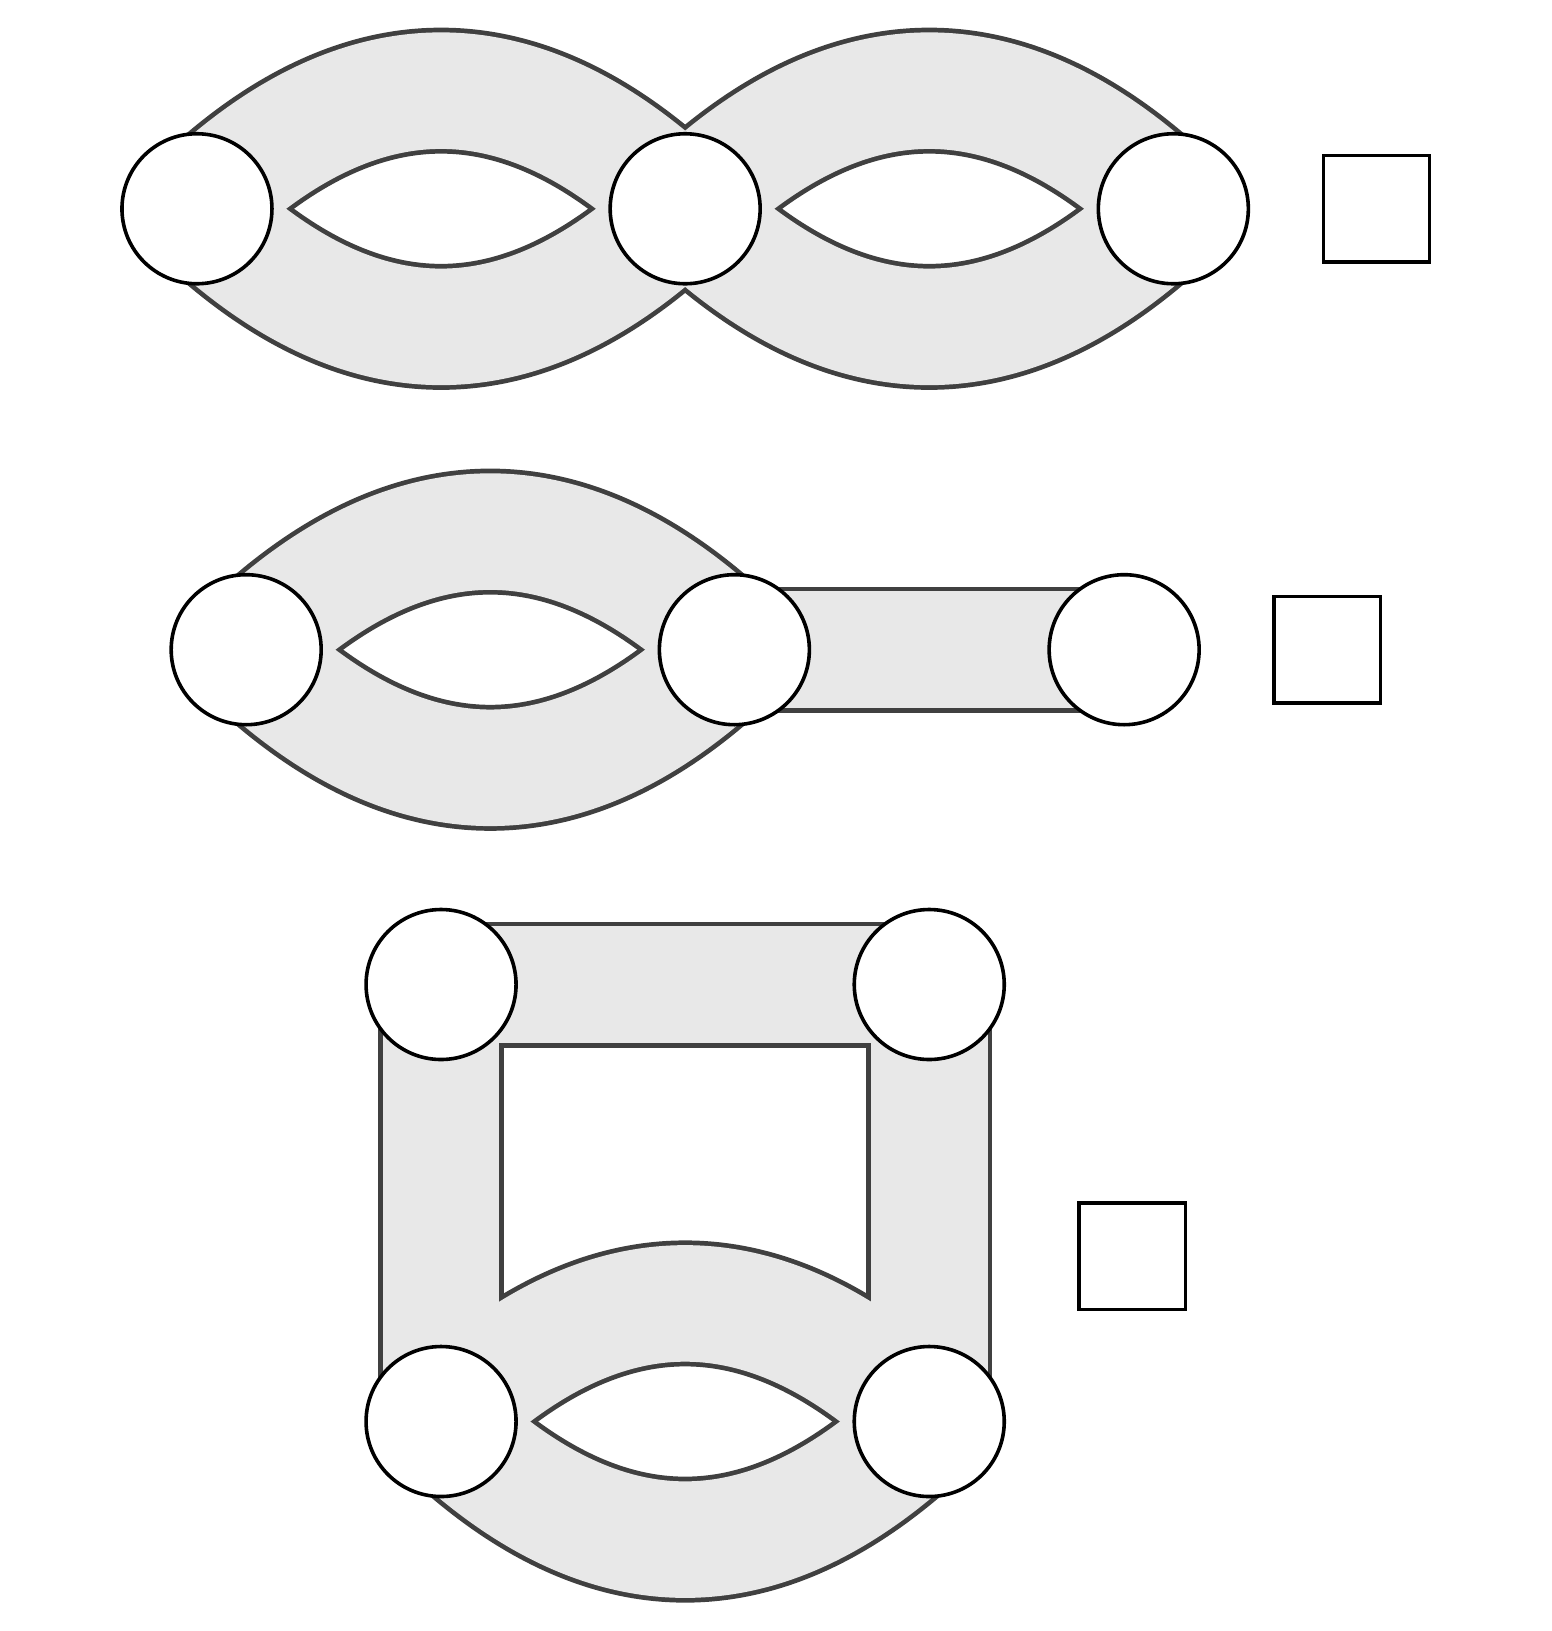
\begin{tikzpicture}
\useasboundingbox (0,0) rectangle (19.0,20.002);
\draw[bandout] (2.150,17.702) .. controls (4.217,19.702) and (6.283,19.702) .. (8.350,17.702);
\draw[bandout] (2.150,17.702) .. controls (4.217,15.702) and (6.283,15.702) .. (8.350,17.702);
\draw[bandout] (8.350,17.702) .. controls (10.417,19.702) and (12.483,19.702) .. (14.550,17.702);
\draw[bandout] (8.350,17.702) .. controls (10.417,15.702) and (12.483,15.702) .. (14.550,17.702);
\draw[bandfill] (2.150,17.702) .. controls (4.217,19.702) and (6.283,19.702) .. (8.350,17.702);
\draw[bandfill] (2.150,17.702) .. controls (4.217,15.702) and (6.283,15.702) .. (8.350,17.702);
\draw[bandfill] (8.350,17.702) .. controls (10.417,19.702) and (12.483,19.702) .. (14.550,17.702);
\draw[bandfill] (8.350,17.702) .. controls (10.417,15.702) and (12.483,15.702) .. (14.550,17.702);
\draw[island] (2.150,17.702) circle (0.9525);
\draw[island] (8.350,17.702) circle (0.9525);
\draw[island] (14.550,17.702) circle (0.9525);
\draw[line width=1.2pt] (16.453,17.027) rectangle ++(1.35,1.35);
\draw[bandout] (2.775,12.102) .. controls (4.842,14.102) and (6.908,14.102) .. (8.975,12.102);
\draw[bandout] (2.775,12.102) .. controls (4.842,10.102) and (6.908,10.102) .. (8.975,12.102);
\draw[bandout] (8.975,12.102) -- (13.925,12.102);
\draw[bandfill] (2.775,12.102) .. controls (4.842,14.102) and (6.908,14.102) .. (8.975,12.102);
\draw[bandfill] (2.775,12.102) .. controls (4.842,10.102) and (6.908,10.102) .. (8.975,12.102);
\draw[bandfill] (8.975,12.102) -- (13.925,12.102);
\draw[island] (2.775,12.102) circle (0.9525);
\draw[island] (8.975,12.102) circle (0.9525);
\draw[island] (13.925,12.102) circle (0.9525);
\draw[line width=1.2pt] (15.828,11.427) rectangle ++(1.35,1.35);
\draw[bandout] (5.250,2.300) .. controls (7.317,4.300) and (9.383,4.300) .. (11.450,2.300);
\draw[bandout] (5.250,2.300) .. controls (7.317,0.300) and (9.383,0.300) .. (11.450,2.300);
\draw[bandout] (11.450,2.300) -- (11.450,7.850);
\draw[bandout] (11.450,7.850) -- (5.250,7.850);
\draw[bandout] (5.250,7.850) -- (5.250,2.300);
\draw[bandfill] (5.250,2.300) .. controls (7.317,4.300) and (9.383,4.300) .. (11.450,2.300);
\draw[bandfill] (5.250,2.300) .. controls (7.317,0.300) and (9.383,0.300) .. (11.450,2.300);
\draw[bandfill] (11.450,2.300) -- (11.450,7.850);
\draw[bandfill] (11.450,7.850) -- (5.250,7.850);
\draw[bandfill] (5.250,7.850) -- (5.250,2.300);
\draw[island] (5.250,2.300) circle (0.9525);
\draw[island] (11.450,2.300) circle (0.9525);
\draw[island] (11.450,7.850) circle (0.9525);
\draw[island] (5.250,7.850) circle (0.9525);
\draw[line width=1.2pt] (13.353,3.726) rectangle ++(1.35,1.35);
\end{tikzpicture}
\end{minipage}


\par\vspace{7mm}\noindent 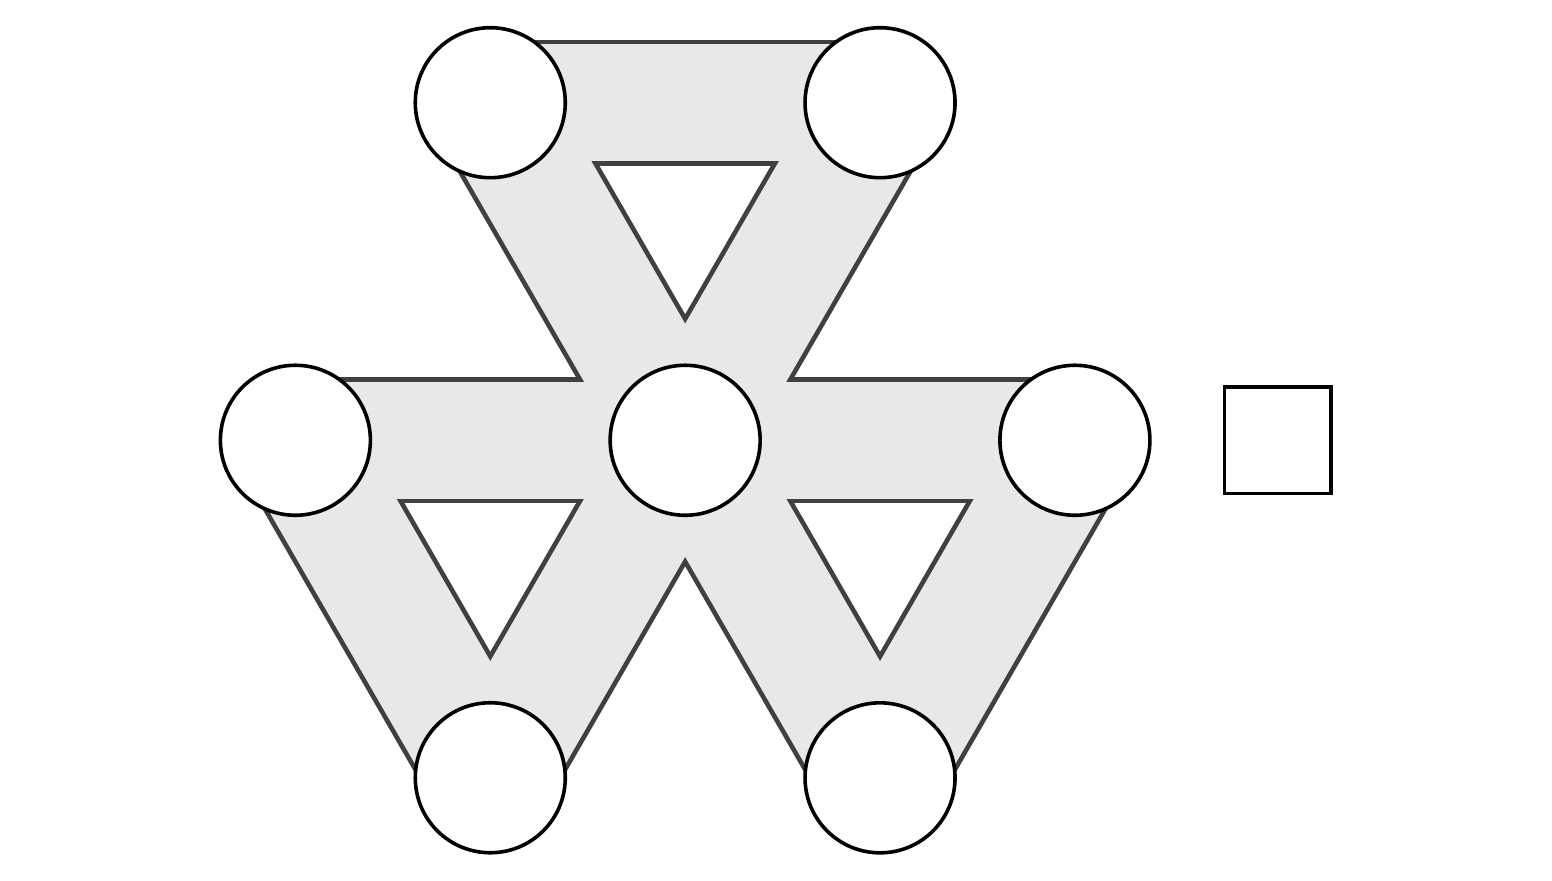
\begin{tikzpicture}
\useasboundingbox (0,0) rectangle (19.0,10.479);
\draw[bandout] (8.350,5.239) -- (10.825,9.526);
\draw[bandout] (10.825,9.526) -- (5.875,9.526);
\draw[bandout] (5.875,9.526) -- (8.350,5.239);
\draw[bandout] (8.350,5.239) -- (3.400,5.239);
\draw[bandout] (3.400,5.239) -- (5.875,0.953);
\draw[bandout] (5.875,0.953) -- (8.350,5.239);
\draw[bandout] (8.350,5.239) -- (10.825,0.952);
\draw[bandout] (10.825,0.952) -- (13.300,5.239);
\draw[bandout] (13.300,5.239) -- (8.350,5.239);
\draw[bandfill] (8.350,5.239) -- (10.825,9.526);
\draw[bandfill] (10.825,9.526) -- (5.875,9.526);
\draw[bandfill] (5.875,9.526) -- (8.350,5.239);
\draw[bandfill] (8.350,5.239) -- (3.400,5.239);
\draw[bandfill] (3.400,5.239) -- (5.875,0.953);
\draw[bandfill] (5.875,0.953) -- (8.350,5.239);
\draw[bandfill] (8.350,5.239) -- (10.825,0.952);
\draw[bandfill] (10.825,0.952) -- (13.300,5.239);
\draw[bandfill] (13.300,5.239) -- (8.350,5.239);
\draw[island] (8.350,5.239) circle (0.9525);
\draw[island] (10.825,9.526) circle (0.9525);
\draw[island] (5.875,9.526) circle (0.9525);
\draw[island] (3.400,5.239) circle (0.9525);
\draw[island] (5.875,0.953) circle (0.9525);
\draw[island] (10.825,0.952) circle (0.9525);
\draw[island] (13.300,5.239) circle (0.9525);
\draw[line width=1.2pt] (15.203,4.564) rectangle ++(1.35,1.35);
\end{tikzpicture}


\par\vspace{7mm}\noindent 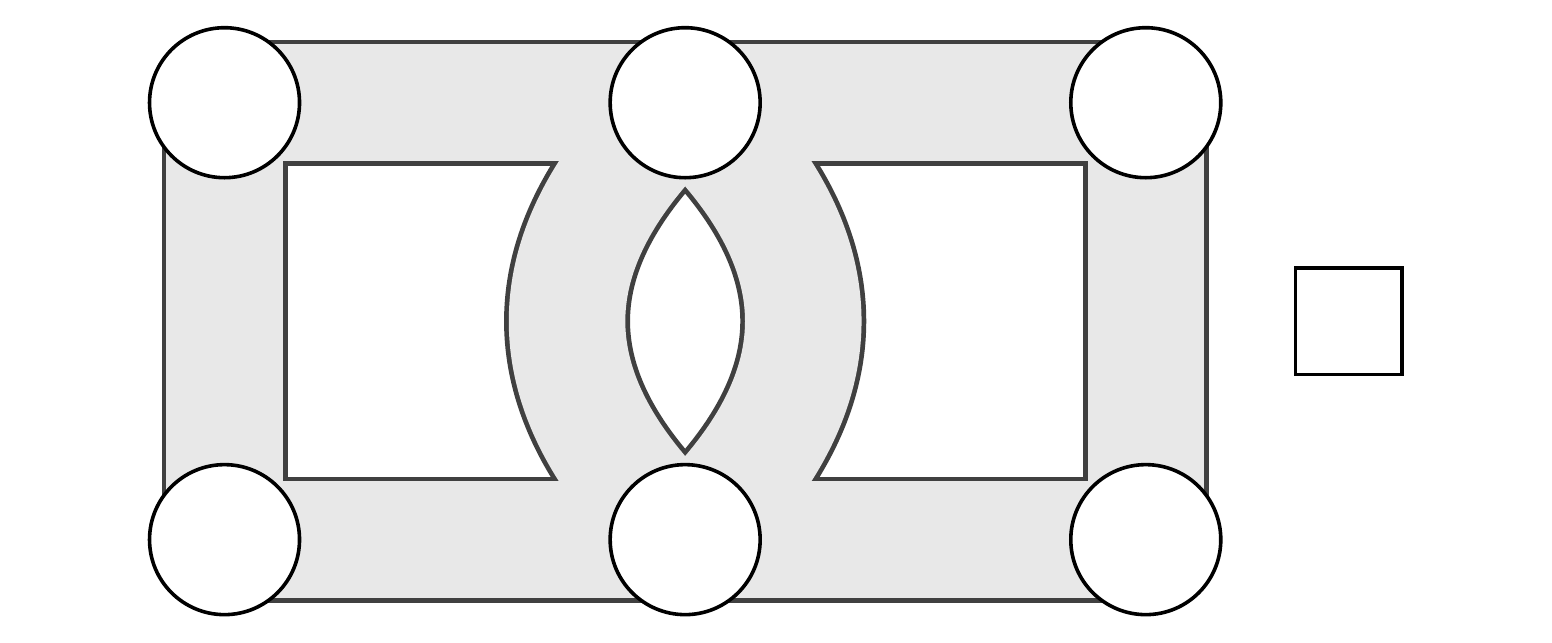
\begin{tikzpicture}
\useasboundingbox (0,0) rectangle (19.0,7.455);
\draw[bandout] (2.500,0.953) -- (8.350,0.953);
\draw[bandout] (2.500,6.502) -- (8.350,6.502);
\draw[bandout] (8.350,0.953) -- (14.200,0.953);
\draw[bandout] (8.350,6.502) -- (14.200,6.502);
\draw[bandout] (2.500,0.953) -- (2.500,6.502);
\draw[bandout] (14.200,0.953) -- (14.200,6.502);
\draw[bandout] (8.350,0.953) .. controls (6.350,2.802) and (6.350,4.652) .. (8.350,6.502);
\draw[bandout] (8.350,0.953) .. controls (10.350,2.802) and (10.350,4.652) .. (8.350,6.502);
\draw[bandfill] (2.500,0.953) -- (8.350,0.953);
\draw[bandfill] (2.500,6.502) -- (8.350,6.502);
\draw[bandfill] (8.350,0.953) -- (14.200,0.953);
\draw[bandfill] (8.350,6.502) -- (14.200,6.502);
\draw[bandfill] (2.500,0.953) -- (2.500,6.502);
\draw[bandfill] (14.200,0.953) -- (14.200,6.502);
\draw[bandfill] (8.350,0.953) .. controls (6.350,2.802) and (6.350,4.652) .. (8.350,6.502);
\draw[bandfill] (8.350,0.953) .. controls (10.350,2.802) and (10.350,4.652) .. (8.350,6.502);
\draw[island] (2.500,0.953) circle (0.9525);
\draw[island] (2.500,6.502) circle (0.9525);
\draw[island] (8.350,0.953) circle (0.9525);
\draw[island] (8.350,6.502) circle (0.9525);
\draw[island] (14.200,0.953) circle (0.9525);
\draw[island] (14.200,6.502) circle (0.9525);
\draw[line width=1.2pt] (16.102,3.052) rectangle ++(1.35,1.35);
\end{tikzpicture}


\par\vspace{9mm}

\newpage

\begin{minipage}{\linewidth}\raggedright
\prob{5}Trace each picture with a colored pencil, without lifting the pencil and without going over a line twice. Cross out each picture that cannot be done.

\vspace{5mm}\noindent 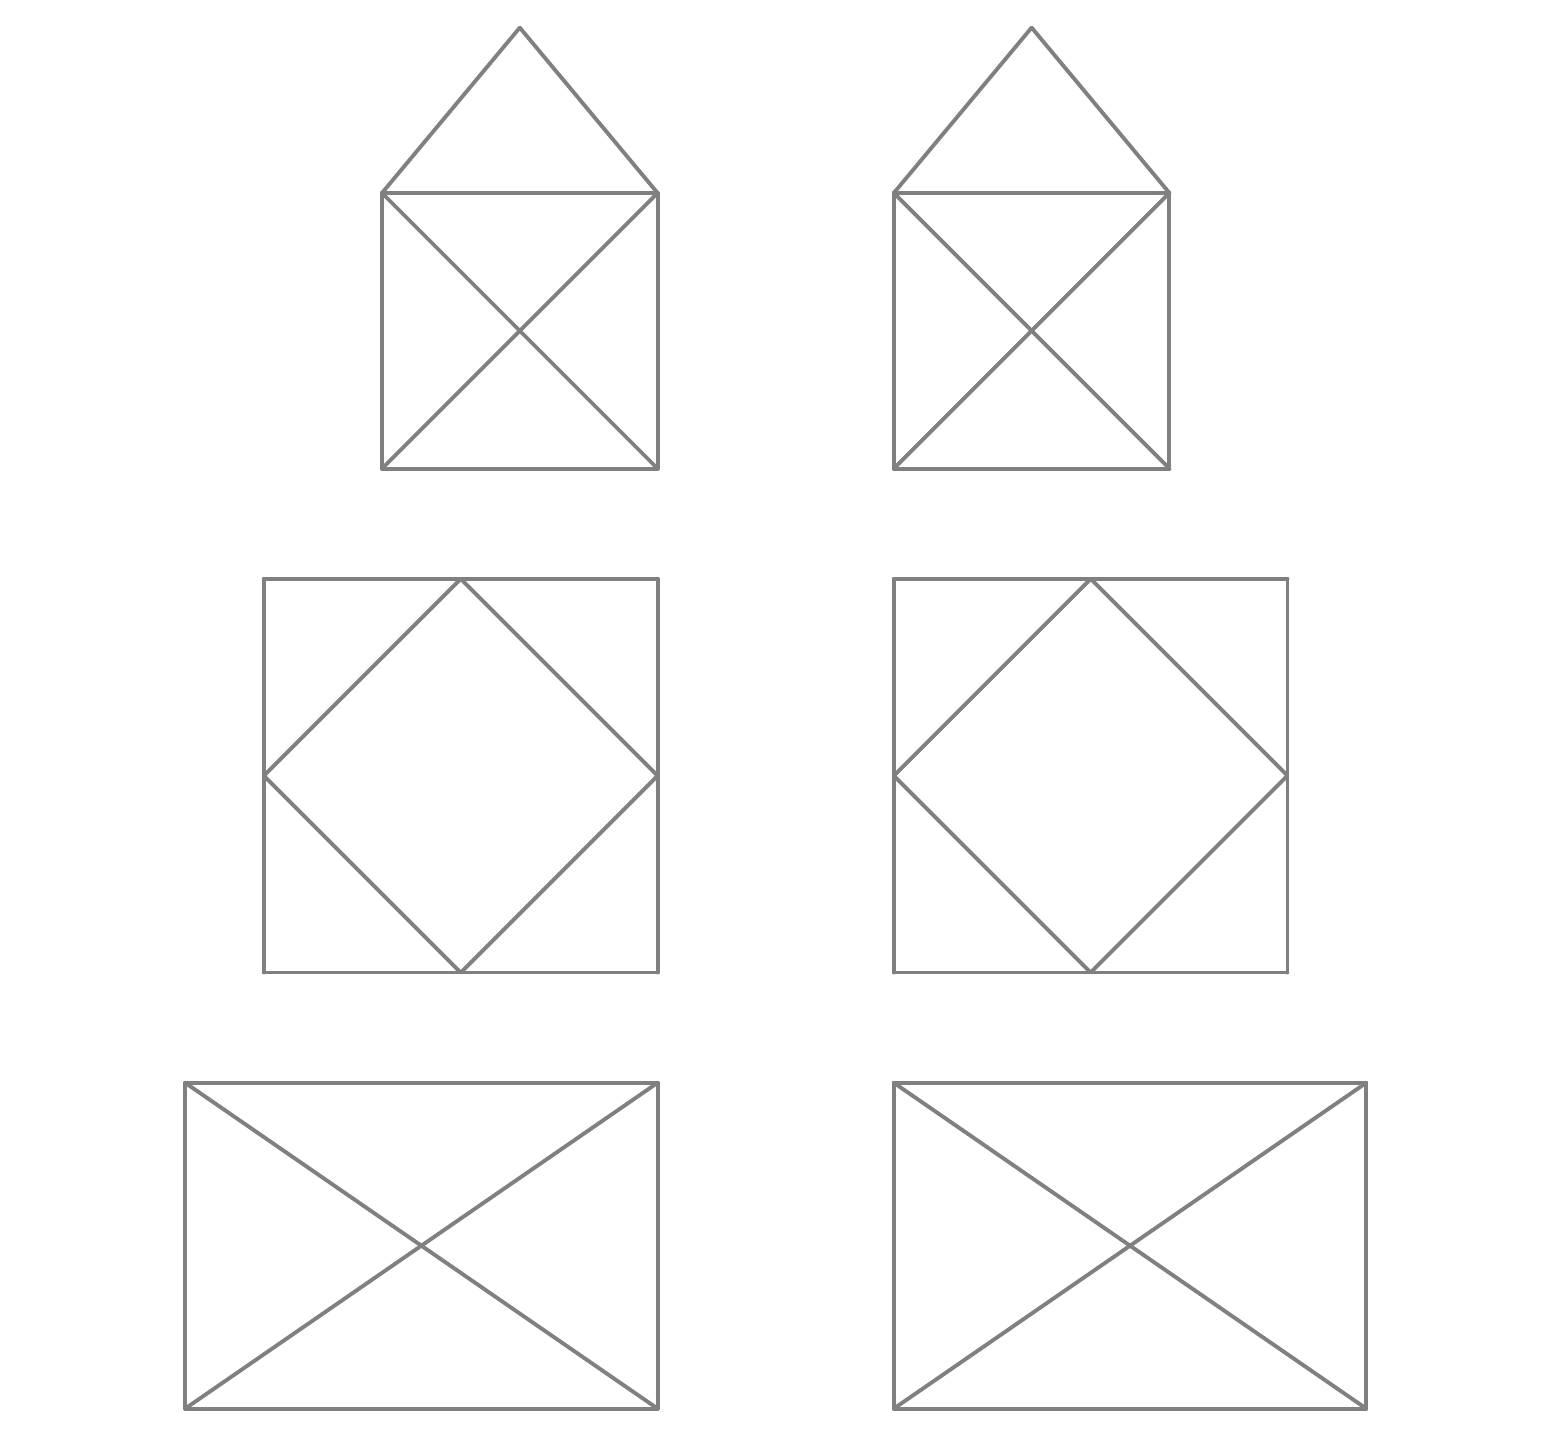
\begin{tikzpicture}
\useasboundingbox (0,0) rectangle (19.0,17.538);
\draw[stroke] (4.500,11.938) -- (8.000,11.938);
\draw[stroke] (8.000,11.938) -- (8.000,15.438);
\draw[stroke] (8.000,15.438) -- (4.500,15.438);
\draw[stroke] (4.500,15.438) -- (4.500,11.938);
\draw[stroke] (4.500,11.938) -- (8.000,15.438);
\draw[stroke] (8.000,11.938) -- (4.500,15.438);
\draw[stroke] (4.500,15.438) -- (6.250,17.538);
\draw[stroke] (6.250,17.538) -- (8.000,15.438);
\draw[stroke] (11.000,11.938) -- (14.500,11.938);
\draw[stroke] (14.500,11.938) -- (14.500,15.438);
\draw[stroke] (14.500,15.438) -- (11.000,15.438);
\draw[stroke] (11.000,15.438) -- (11.000,11.938);
\draw[stroke] (11.000,11.938) -- (14.500,15.438);
\draw[stroke] (14.500,11.938) -- (11.000,15.438);
\draw[stroke] (11.000,15.438) -- (12.750,17.538);
\draw[stroke] (12.750,17.538) -- (14.500,15.438);
\draw[stroke] (3.000,5.538) -- (8.000,5.538);
\draw[stroke] (8.000,5.538) -- (8.000,10.538);
\draw[stroke] (8.000,10.538) -- (3.000,10.538);
\draw[stroke] (3.000,10.538) -- (3.000,5.538);
\draw[stroke] (5.500,5.538) -- (8.000,8.038);
\draw[stroke] (8.000,8.038) -- (5.500,10.538);
\draw[stroke] (5.500,10.538) -- (3.000,8.038);
\draw[stroke] (3.000,8.038) -- (5.500,5.538);
\draw[stroke] (11.000,5.538) -- (16.000,5.538);
\draw[stroke] (16.000,5.538) -- (16.000,10.538);
\draw[stroke] (16.000,10.538) -- (11.000,10.538);
\draw[stroke] (11.000,10.538) -- (11.000,5.538);
\draw[stroke] (13.500,5.538) -- (16.000,8.038);
\draw[stroke] (16.000,8.038) -- (13.500,10.538);
\draw[stroke] (13.500,10.538) -- (11.000,8.038);
\draw[stroke] (11.000,8.038) -- (13.500,5.538);
\draw[stroke] (2.000,0.000) -- (8.000,0.000);
\draw[stroke] (8.000,0.000) -- (8.000,4.138);
\draw[stroke] (8.000,4.138) -- (2.000,4.138);
\draw[stroke] (2.000,4.138) -- (2.000,0.000);
\draw[stroke] (2.000,0.000) -- (8.000,4.138);
\draw[stroke] (8.000,0.000) -- (2.000,4.138);
\draw[stroke] (11.000,0.000) -- (17.000,0.000);
\draw[stroke] (17.000,0.000) -- (17.000,4.138);
\draw[stroke] (17.000,4.138) -- (11.000,4.138);
\draw[stroke] (11.000,4.138) -- (11.000,0.000);
\draw[stroke] (11.000,0.000) -- (17.000,4.138);
\draw[stroke] (17.000,0.000) -- (11.000,4.138);
\end{tikzpicture}
\end{minipage}


\par\vspace{7mm}\noindent 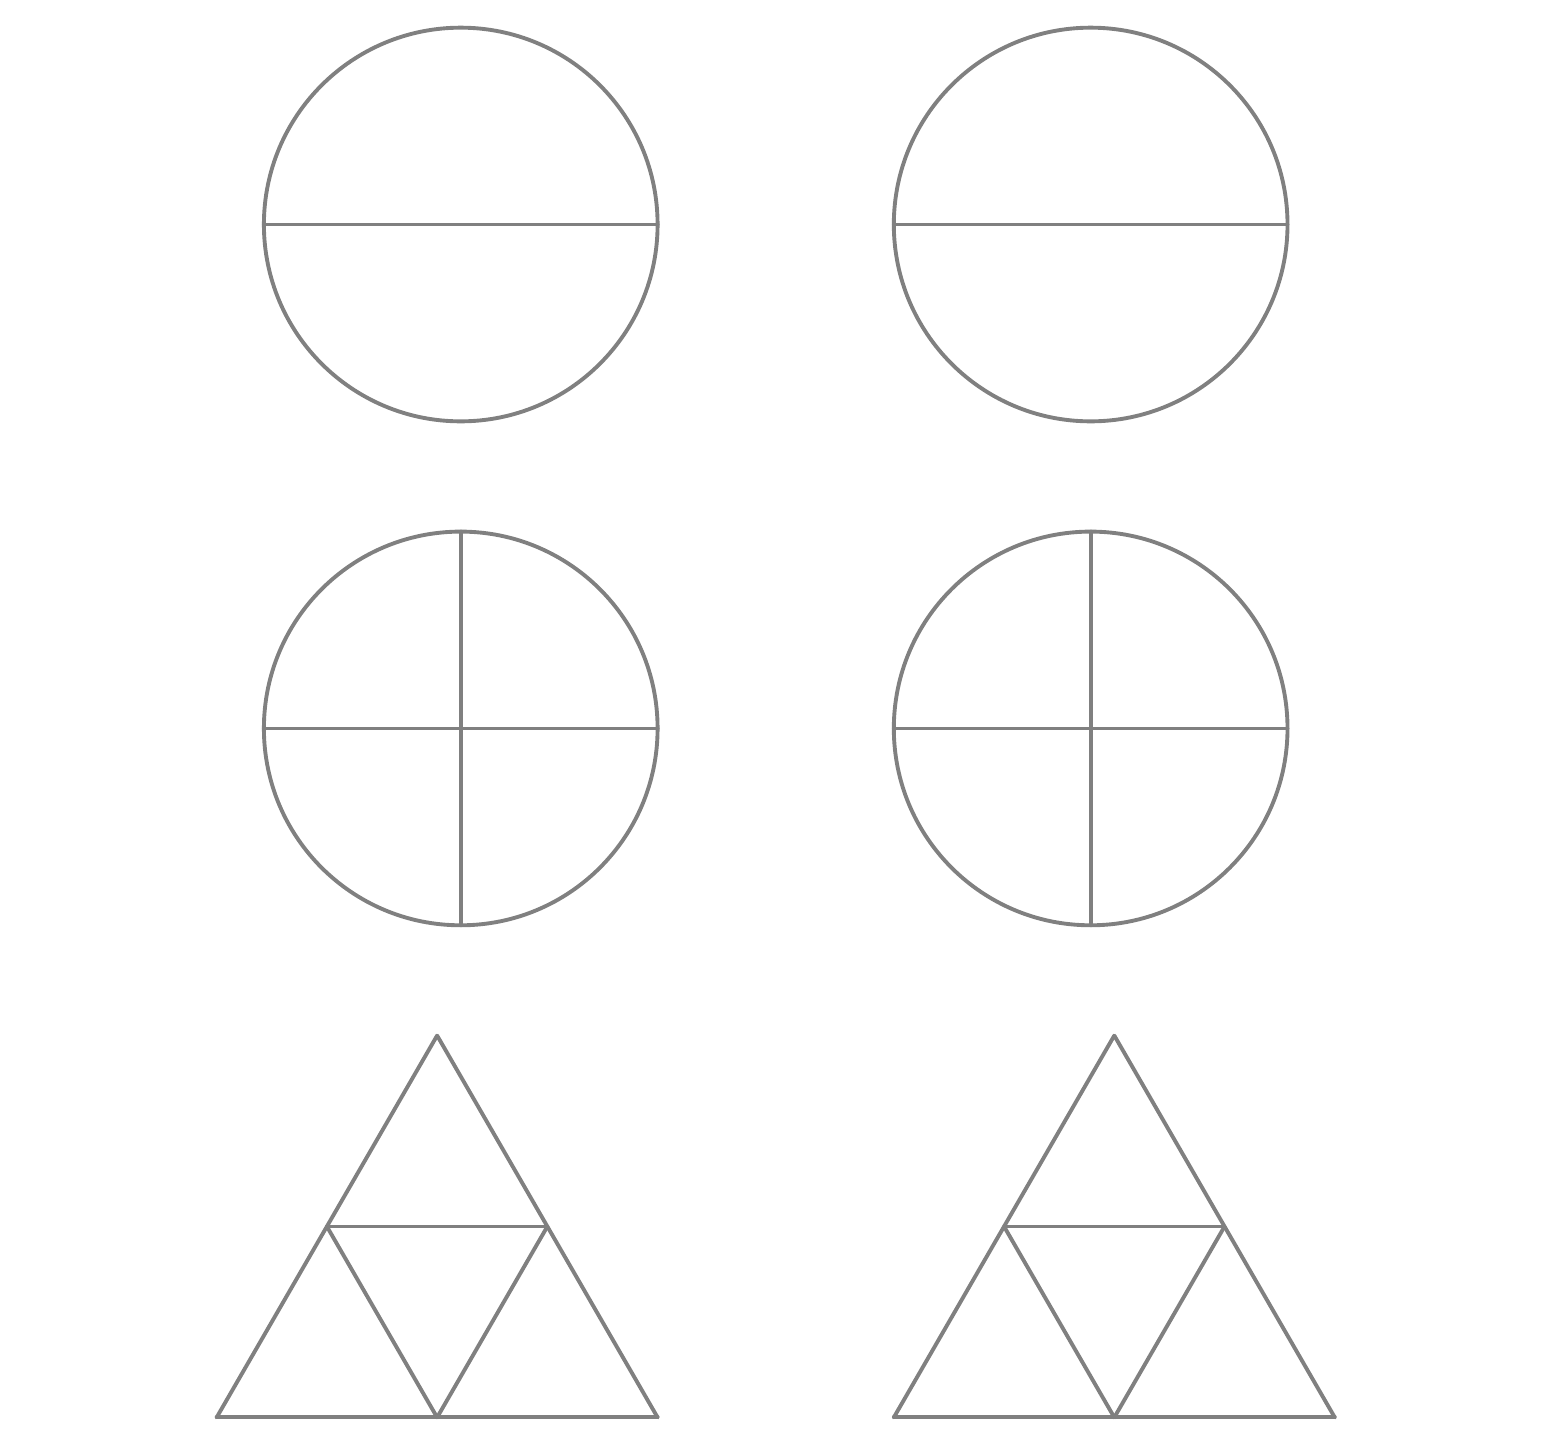
\begin{tikzpicture}
\useasboundingbox (0,0) rectangle (19.0,17.650);
\draw[stroke] (3.000,15.150) -- (8.000,15.150);
\draw[stroke] (5.500,15.150) circle (2.500);
\draw[stroke] (11.000,15.150) -- (16.000,15.150);
\draw[stroke] (13.500,15.150) circle (2.500);
\draw[stroke] (3.000,8.750) -- (8.000,8.750);
\draw[stroke] (5.500,6.250) -- (5.500,11.250);
\draw[stroke] (5.500,8.750) circle (2.500);
\draw[stroke] (11.000,8.750) -- (16.000,8.750);
\draw[stroke] (13.500,6.250) -- (13.500,11.250);
\draw[stroke] (13.500,8.750) circle (2.500);
\draw[stroke] (2.400,-0.000) -- (8.000,-0.000);
\draw[stroke] (8.000,-0.000) -- (5.200,4.850);
\draw[stroke] (5.200,4.850) -- (2.400,-0.000);
\draw[stroke] (5.200,-0.000) -- (6.600,2.425);
\draw[stroke] (6.600,2.425) -- (3.800,2.425);
\draw[stroke] (3.800,2.425) -- (5.200,-0.000);
\draw[stroke] (11.000,-0.000) -- (16.600,-0.000);
\draw[stroke] (16.600,-0.000) -- (13.800,4.850);
\draw[stroke] (13.800,4.850) -- (11.000,-0.000);
\draw[stroke] (13.800,-0.000) -- (15.200,2.425);
\draw[stroke] (15.200,2.425) -- (12.400,2.425);
\draw[stroke] (12.400,2.425) -- (13.800,-0.000);
\end{tikzpicture}


\par\vspace{9mm}

\newpage

\begin{minipage}{\linewidth}\raggedright
\prob{6}Nobody can pick up every counter in these towns. Draw one more bridge in each town so that you can.

\vspace{5mm}\noindent 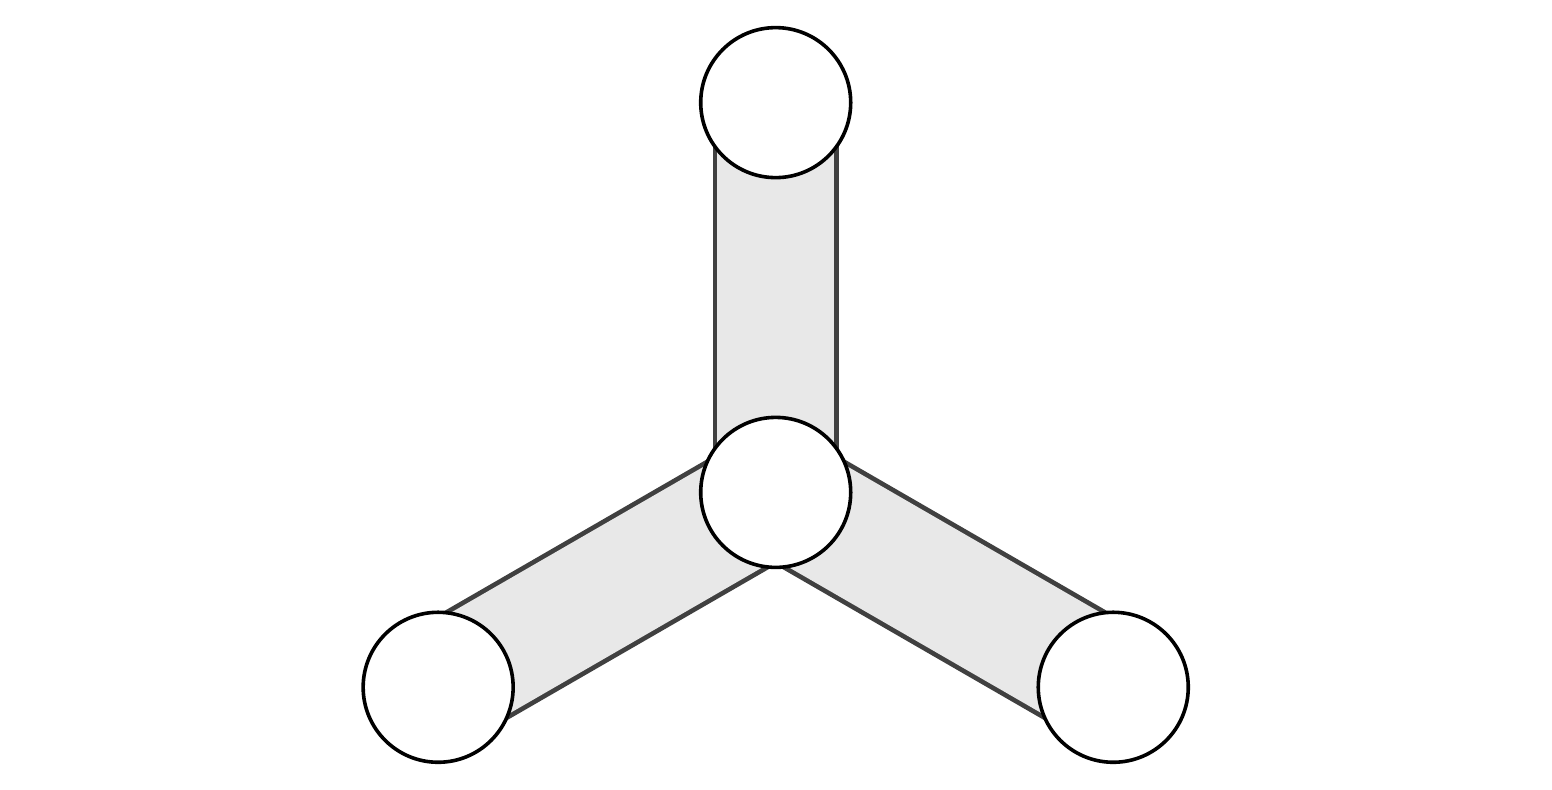
\begin{tikzpicture}
\useasboundingbox (0,0) rectangle (19.0,9.330);
\draw[bandout] (9.500,3.428) -- (9.500,8.378);
\draw[bandout] (9.500,3.428) -- (5.213,0.953);
\draw[bandout] (9.500,3.428) -- (13.787,0.953);
\draw[bandfill] (9.500,3.428) -- (9.500,8.378);
\draw[bandfill] (9.500,3.428) -- (5.213,0.953);
\draw[bandfill] (9.500,3.428) -- (13.787,0.953);
\draw[island] (9.500,3.428) circle (0.9525);
\draw[island] (9.500,8.378) circle (0.9525);
\draw[island] (5.213,0.953) circle (0.9525);
\draw[island] (13.787,0.953) circle (0.9525);
\end{tikzpicture}
\end{minipage}


\par\vspace{7mm}\noindent 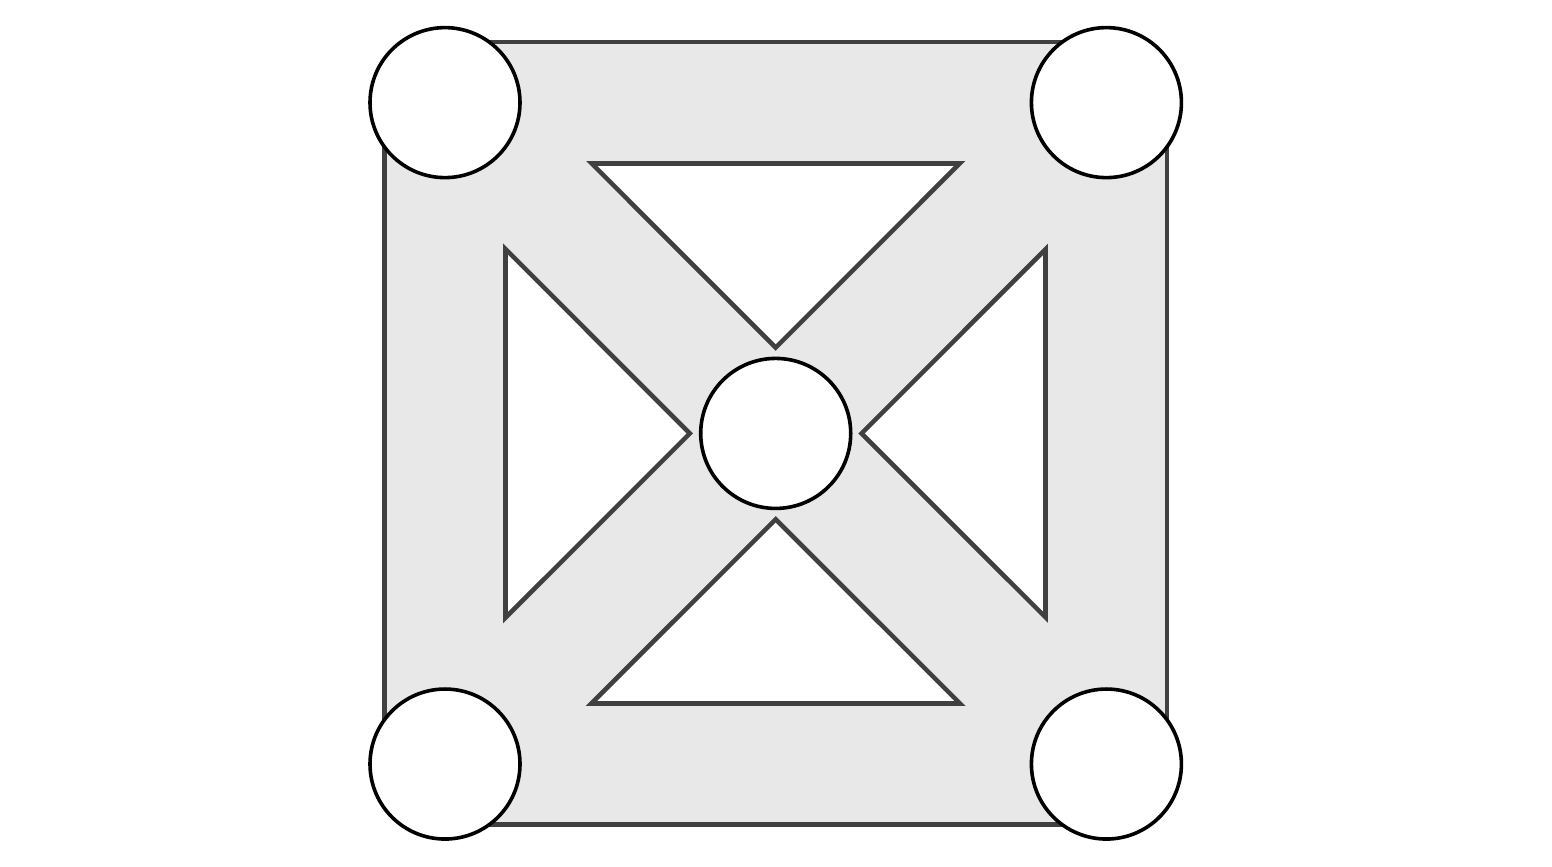
\begin{tikzpicture}
\useasboundingbox (0,0) rectangle (19.0,10.305);
\draw[bandout] (5.300,0.953) -- (13.700,0.953);
\draw[bandout] (13.700,0.953) -- (13.700,9.353);
\draw[bandout] (13.700,9.353) -- (5.300,9.353);
\draw[bandout] (5.300,9.353) -- (5.300,0.953);
\draw[bandout] (9.500,5.152) -- (5.300,0.953);
\draw[bandout] (9.500,5.152) -- (13.700,0.953);
\draw[bandout] (9.500,5.152) -- (13.700,9.353);
\draw[bandout] (9.500,5.152) -- (5.300,9.353);
\draw[bandfill] (5.300,0.953) -- (13.700,0.953);
\draw[bandfill] (13.700,0.953) -- (13.700,9.353);
\draw[bandfill] (13.700,9.353) -- (5.300,9.353);
\draw[bandfill] (5.300,9.353) -- (5.300,0.953);
\draw[bandfill] (9.500,5.152) -- (5.300,0.953);
\draw[bandfill] (9.500,5.152) -- (13.700,0.953);
\draw[bandfill] (9.500,5.152) -- (13.700,9.353);
\draw[bandfill] (9.500,5.152) -- (5.300,9.353);
\draw[island] (5.300,0.953) circle (0.9525);
\draw[island] (13.700,0.953) circle (0.9525);
\draw[island] (13.700,9.353) circle (0.9525);
\draw[island] (5.300,9.353) circle (0.9525);
\draw[island] (9.500,5.152) circle (0.9525);
\end{tikzpicture}


\par\vspace{7mm}\noindent 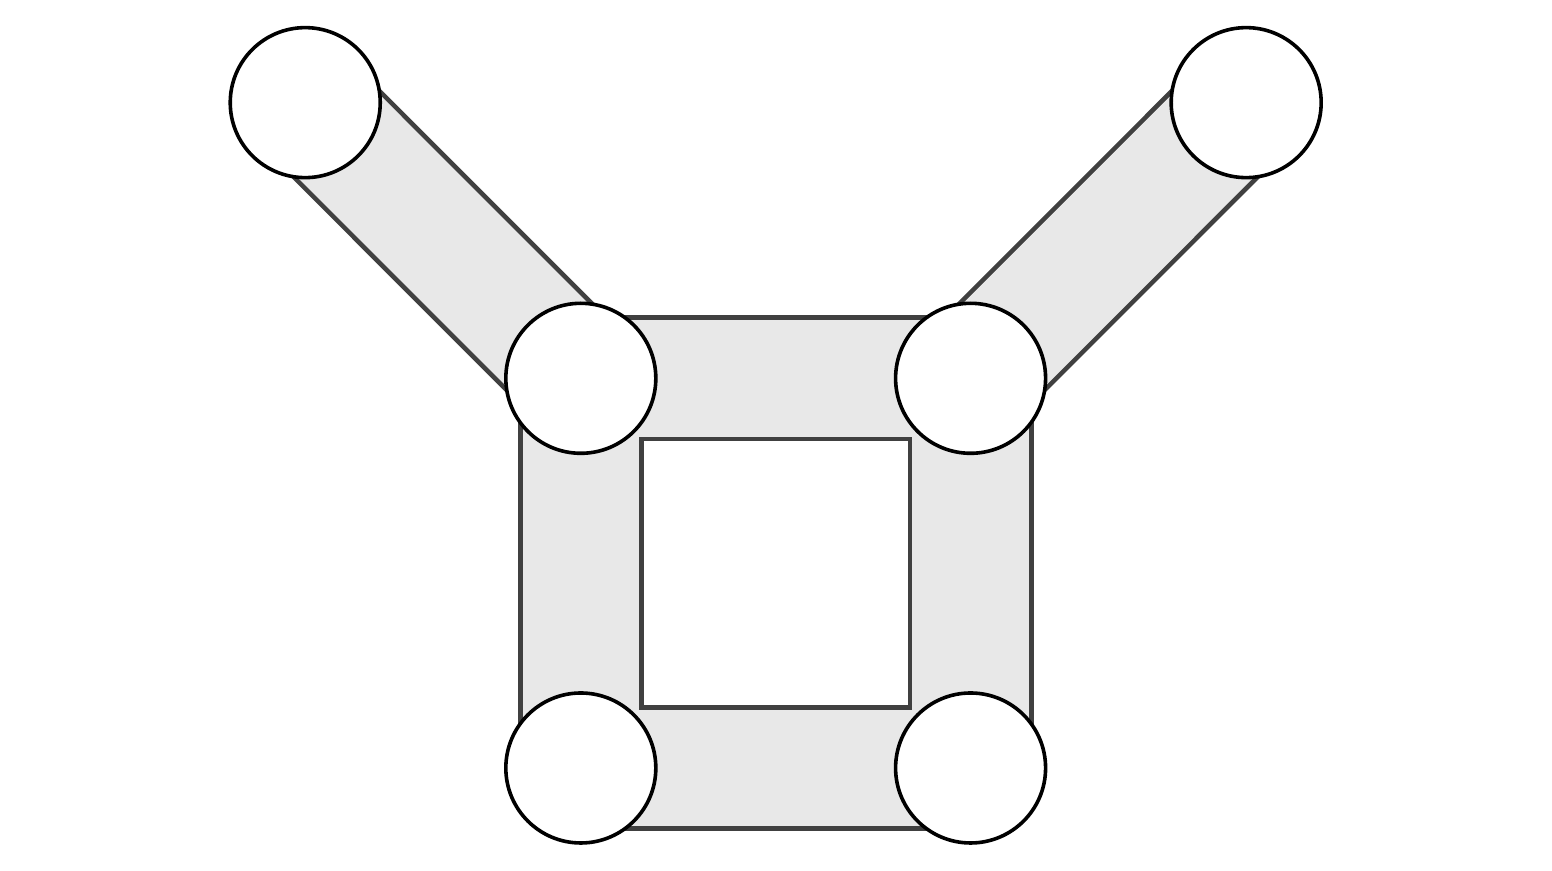
\begin{tikzpicture}
\useasboundingbox (0,0) rectangle (19.0,10.355);
\draw[bandout] (7.025,0.953) -- (11.975,0.953);
\draw[bandout] (11.975,0.953) -- (11.975,5.902);
\draw[bandout] (11.975,5.902) -- (7.025,5.902);
\draw[bandout] (7.025,5.902) -- (7.025,0.953);
\draw[bandout] (7.025,5.902) -- (3.525,9.403);
\draw[bandout] (11.975,5.902) -- (15.475,9.403);
\draw[bandfill] (7.025,0.953) -- (11.975,0.953);
\draw[bandfill] (11.975,0.953) -- (11.975,5.902);
\draw[bandfill] (11.975,5.902) -- (7.025,5.902);
\draw[bandfill] (7.025,5.902) -- (7.025,0.953);
\draw[bandfill] (7.025,5.902) -- (3.525,9.403);
\draw[bandfill] (11.975,5.902) -- (15.475,9.403);
\draw[island] (7.025,0.953) circle (0.9525);
\draw[island] (11.975,0.953) circle (0.9525);
\draw[island] (11.975,5.902) circle (0.9525);
\draw[island] (7.025,5.902) circle (0.9525);
\draw[island] (3.525,9.403) circle (0.9525);
\draw[island] (15.475,9.403) circle (0.9525);
\end{tikzpicture}


\par\vspace{9mm}

\begin{minipage}{\linewidth}\raggedright
\prob{7}Join 4 hexagons with craft sticks into one town where your partner can pick up every counter. Then make a town of 4 joined hexagons where your partner cannot, and draw both towns.

\vspace{5mm}\noindent \begin{tikzpicture}
\useasboundingbox (0,0) rectangle (19.0,9.000);
\draw[line width=0.9pt, black!70] (0.000,0.000) rectangle ++(9.0,9.0);
\draw[line width=0.9pt, black!70] (10.000,0.000) rectangle ++(9.0,9.0);
\end{tikzpicture}
\end{minipage}


\par\vspace{9mm}

\newpage

\begin{minipage}{\linewidth}\raggedright
\prob{8}Put two counters on one bridge and try to pick up every counter. Color each bridge where that works.

\vspace{5mm}\noindent 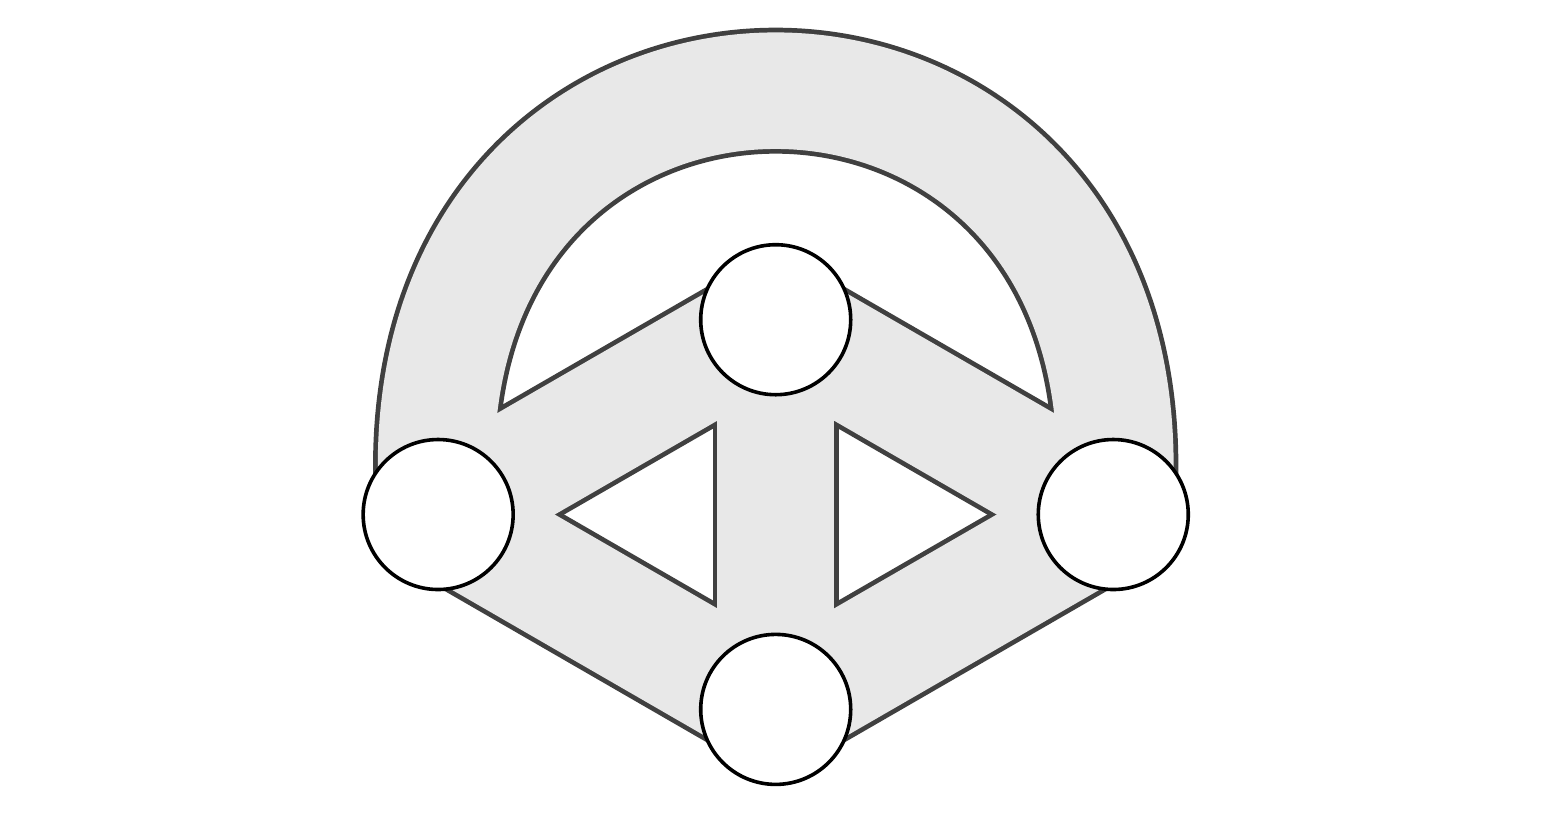
\begin{tikzpicture}
\useasboundingbox (0,0) rectangle (19.0,9.611);
\draw[bandout] (9.500,5.902) -- (9.500,0.953);
\draw[bandout] (9.500,5.902) -- (5.213,3.428);
\draw[bandout] (9.500,5.902) -- (13.787,3.428);
\draw[bandout] (9.500,0.953) -- (5.213,3.428);
\draw[bandout] (9.500,0.953) -- (13.787,3.428);
\draw[bandout] (5.213,3.428) .. controls (4.613,10.605) and (14.387,10.605) .. (13.787,3.428);
\draw[bandfill] (9.500,5.902) -- (9.500,0.953);
\draw[bandfill] (9.500,5.902) -- (5.213,3.428);
\draw[bandfill] (9.500,5.902) -- (13.787,3.428);
\draw[bandfill] (9.500,0.953) -- (5.213,3.428);
\draw[bandfill] (9.500,0.953) -- (13.787,3.428);
\draw[bandfill] (5.213,3.428) .. controls (4.613,10.605) and (14.387,10.605) .. (13.787,3.428);
\draw[island] (9.500,5.902) circle (0.9525);
\draw[island] (9.500,0.953) circle (0.9525);
\draw[island] (5.213,3.428) circle (0.9525);
\draw[island] (13.787,3.428) circle (0.9525);
\end{tikzpicture}
\end{minipage}


\par\vspace{7mm}\noindent 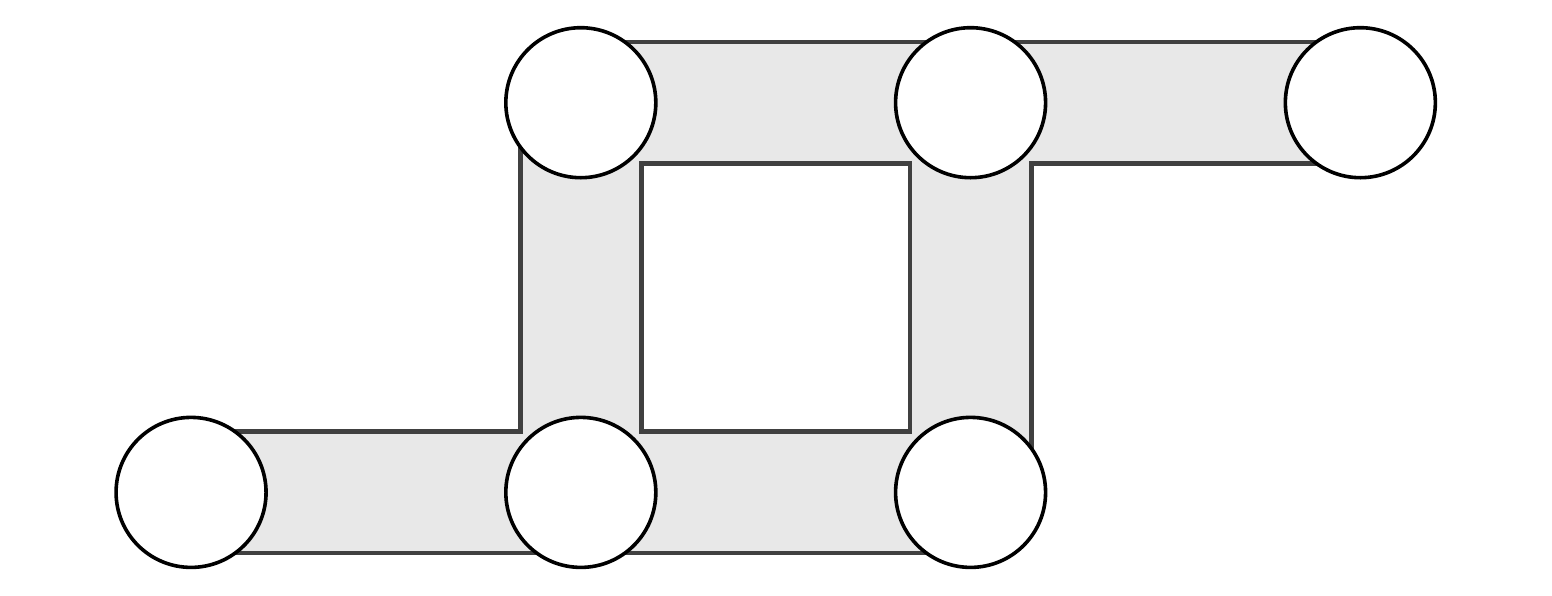
\begin{tikzpicture}
\useasboundingbox (0,0) rectangle (19.0,6.855);
\draw[bandout] (7.025,0.953) -- (11.975,0.953);
\draw[bandout] (11.975,0.953) -- (11.975,5.902);
\draw[bandout] (11.975,5.902) -- (7.025,5.902);
\draw[bandout] (7.025,5.902) -- (7.025,0.953);
\draw[bandout] (2.075,0.953) -- (7.025,0.953);
\draw[bandout] (11.975,5.902) -- (16.925,5.902);
\draw[bandfill] (7.025,0.953) -- (11.975,0.953);
\draw[bandfill] (11.975,0.953) -- (11.975,5.902);
\draw[bandfill] (11.975,5.902) -- (7.025,5.902);
\draw[bandfill] (7.025,5.902) -- (7.025,0.953);
\draw[bandfill] (2.075,0.953) -- (7.025,0.953);
\draw[bandfill] (11.975,5.902) -- (16.925,5.902);
\draw[island] (7.025,0.953) circle (0.9525);
\draw[island] (11.975,0.953) circle (0.9525);
\draw[island] (11.975,5.902) circle (0.9525);
\draw[island] (7.025,5.902) circle (0.9525);
\draw[island] (2.075,0.953) circle (0.9525);
\draw[island] (16.925,5.902) circle (0.9525);
\end{tikzpicture}


\par\vspace{7mm}\noindent 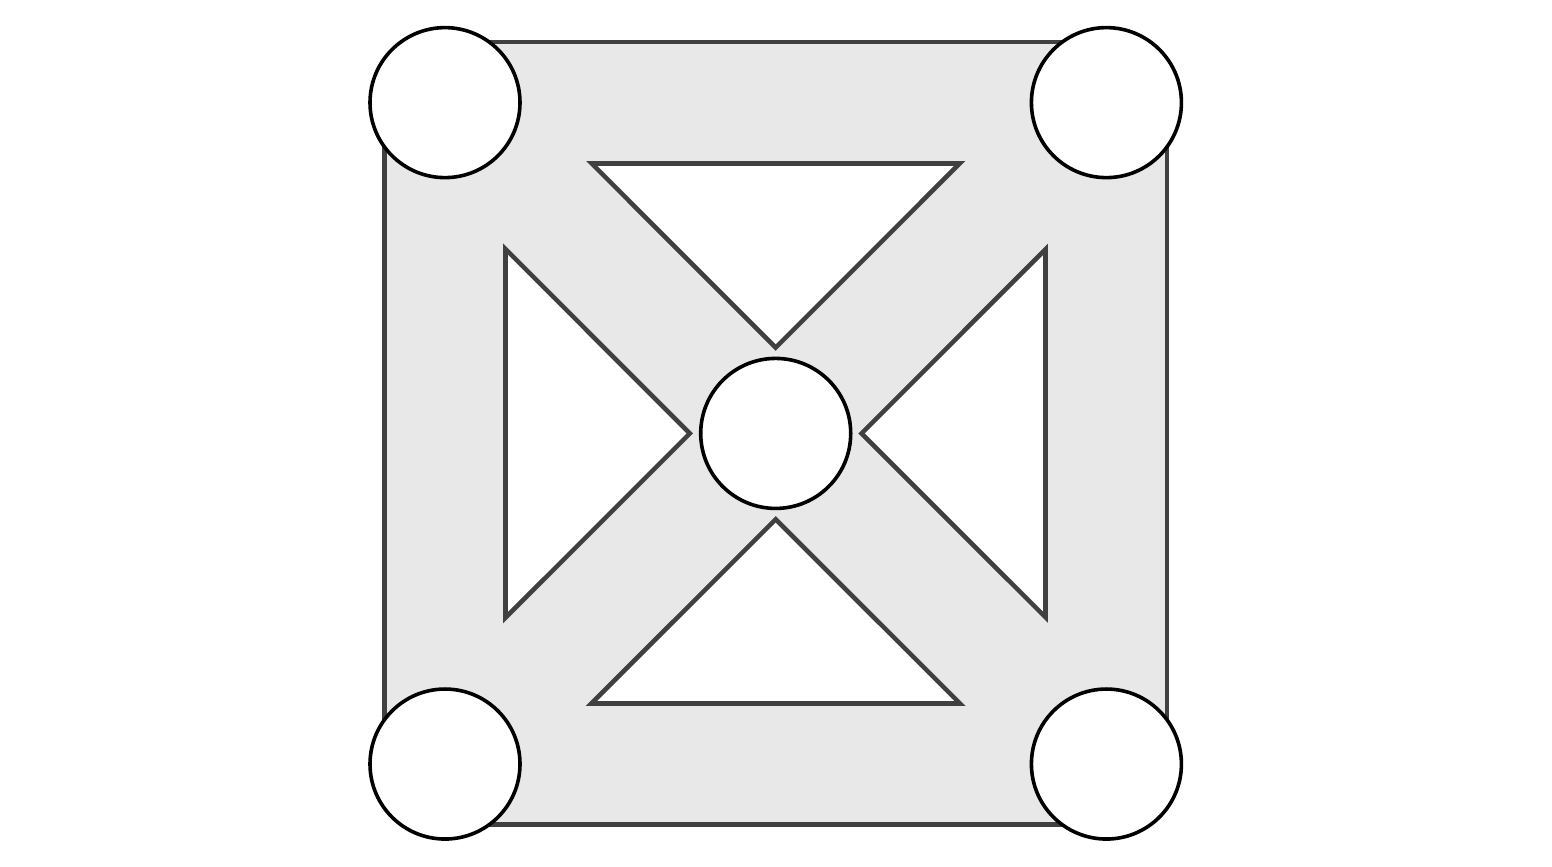
\begin{tikzpicture}
\useasboundingbox (0,0) rectangle (19.0,10.305);
\draw[bandout] (5.300,0.953) -- (13.700,0.953);
\draw[bandout] (13.700,0.953) -- (13.700,9.353);
\draw[bandout] (13.700,9.353) -- (5.300,9.353);
\draw[bandout] (5.300,9.353) -- (5.300,0.953);
\draw[bandout] (9.500,5.152) -- (5.300,0.953);
\draw[bandout] (9.500,5.152) -- (13.700,0.953);
\draw[bandout] (9.500,5.152) -- (13.700,9.353);
\draw[bandout] (9.500,5.152) -- (5.300,9.353);
\draw[bandfill] (5.300,0.953) -- (13.700,0.953);
\draw[bandfill] (13.700,0.953) -- (13.700,9.353);
\draw[bandfill] (13.700,9.353) -- (5.300,9.353);
\draw[bandfill] (5.300,9.353) -- (5.300,0.953);
\draw[bandfill] (9.500,5.152) -- (5.300,0.953);
\draw[bandfill] (9.500,5.152) -- (13.700,0.953);
\draw[bandfill] (9.500,5.152) -- (13.700,9.353);
\draw[bandfill] (9.500,5.152) -- (5.300,9.353);
\draw[island] (5.300,0.953) circle (0.9525);
\draw[island] (13.700,0.953) circle (0.9525);
\draw[island] (13.700,9.353) circle (0.9525);
\draw[island] (5.300,9.353) circle (0.9525);
\draw[island] (9.500,5.152) circle (0.9525);
\end{tikzpicture}


\par\vspace{9mm}
\end{document}
